
\documentclass[12p]{article}
\usepackage{latexsym}
\usepackage{lmodern}
\usepackage[T1]{fontenc}
\usepackage[spanish,activeacute]{babel}
\usepackage[utf8]{inputenc}
\usepackage{mathtools}
\usepackage{amssymb}
\usepackage{amsmath}
\usepackage{graphicx}
\usepackage{hyperref}
\usepackage{listings}
\graphicspath{{Imagenes/}}
\usepackage[export]{adjustbox}[2011/08/13]

\setlength{\oddsidemargin}{-0.25in}
\setlength{\textwidth}{7in}
\setlength{\topmargin}{-.75in}
\setlength{\textheight}{9.2in}
\setlength{\parindent}{1cm}
\setlength{\parskip}{1ex}

\renewcommand{\baselinestretch}{1}\usepackage{lmodern}
\usepackage{listings} 
\usepackage{enumerate} 


\title{Dinámica de una partícula en un aro giratorio como experimento para estudiantes de licenciatura}
\author
{Barr\'on Jim\'enez, Isaac
	\and
	G\'omez Arias, Andr\'es
	\and
	Nellen Mondrag\'on, Stefan Daniel
	\and
	S\'anchez Alvarado, Sergio Jonathan	
	}
\date{\today}

\begin{document}
\maketitle

\abstract 
{Se realizan múltiples análisis exhaustivos para obtener los puntos de equilibrio de una partícula en un aro en rotación, y los parámetros de los cuales dependen, así como sus propiedades. Se utilizan diversos métodos de análisis teórico, desde el análisis de fuerzas, la formulación de Lagrange, hasta el análisis del potencial efectivo, llegando a los mismos resultados. Se comprueba exitósamente lo obtenido teóricamente, por lo que se comprueban experimentalmente y al mismo tiempo las 3 formulaciones utilizadas. Incluso se obtiene un experimento en particular con una fenomenología muy característica, donde la partícula mantiene oscilaciones dentro del aro cuyo periodo coincide con el periodo de rotación del aro. 
}
\newpage


\section{Introducción}
El sistema físico consta de un aro circular que es rotado verticalmente con velocidad angular constante, con eje de giro como su diámetro. Dentro del aro, restringido por una barrera, se coloca una masa pequeña con poca fricción. Se coloca una cámara en un tripié para gravar el movimiento de la partícula, lo que sólo permite que existan mediciones con una diferencia de tiempo de la mitad del periodo de rotación. Es decir, cuando el aro está alineado con el plano dado por el video, donde no hay errores de perspectiva con respecto al patrón de medición, colocado en dicho plano.
Se observa y se mide el movimiento de la partícula en cada momento posible y la altura máxima a la que llega la partícula para diferentes velocidades angulares, pero cada una constante.

Obsérvese el diagrama, en él que se denotan las variables que se van a utilizar.

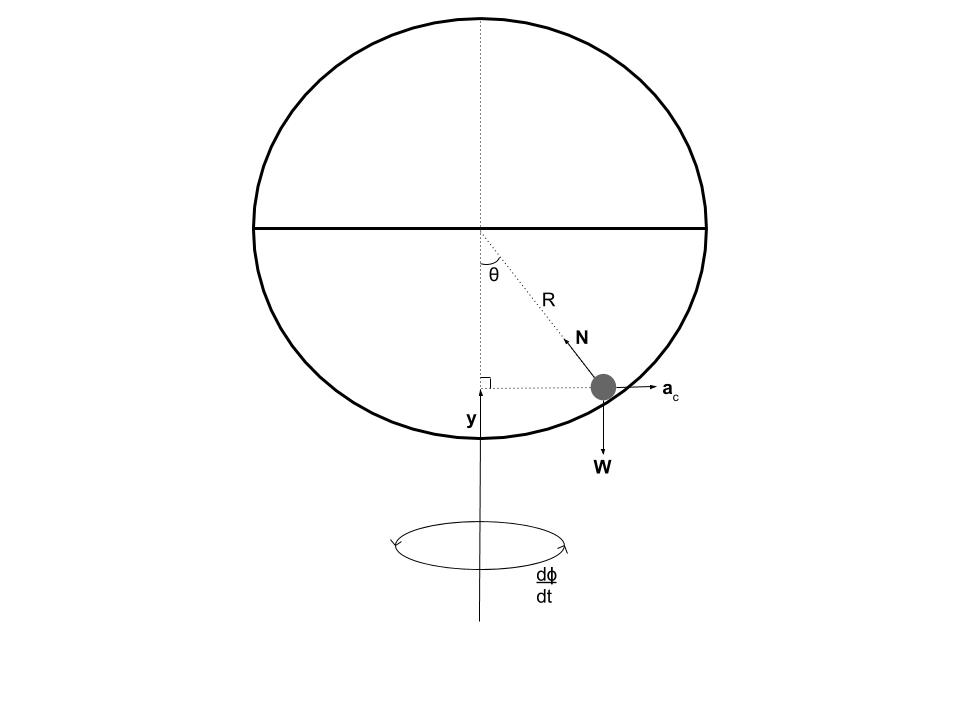
\includegraphics[scale=0.38,center]{Diagrama}

Siguiendo el diagrama de cuerpo libre sobre la partícula en el interior del aro que gira, tenemos que:
$$-Nsen(\theta)=ma_{c}=m(\ddot{r}-r\dot{\phi}^2)$$
donde $\phi$ corresponde al ángulo de giro del aro y $r$ es la distancia del eje de giro a la partícula.

en la dirección horizontal radial, donde $\phi$ corresponde al ángulo de giro del aro y $r$ es la distancia del eje de giro a la partícula.

$$Ncos(\theta)-mg=m\ddot{y}$$
en la dirección vertical.

Cuando la bola llega a su altura máxima, y asumiendo que la bola no puede alcanzar una altura mayor que el radio $R$: $\ddot{y}=0$, $\ddot{r}=0$ y $y=h_{m}$
Entonces
$$Nsen(\theta)=mr\dot{\phi}^2$$
y
$$ N=\frac{m}{cos(\theta)}g$$ 

Sustituyendo N:

$$gtan(\theta)=g\frac{r}{R-h_{m}}=r\dot{\phi}^2$$

Por lo que

\begin{equation}
h_{m}=R-\frac{g}{\dot{\phi}^2}
\end{equation}

La cual sólo tiene sentido cuando 
$$\dot{\phi} \geq \sqrt{\frac{g}{R}}$$

Es decir, $\sqrt{g}{R}$ nos da un valor crítico de la velocidad angular. Para velocidades angulares menores, no debería haber elevación, y para velocidades angulares mayores se espera una elevación.

Por otra parte, podemos utilizar la formulación lagrangiana para llegar a una ecuación diferencial de ángulo con respecto al tiempo, y a partir de ahí encontrar más información que sólo con el análisis de fuerzas.

La velocidad de la partícula en coordenadas esféricas está dada por:

$$\dot{\vec{r}}=\dot{r}\hat{r}+r\theta\hat{\theta}+rsin(\theta)\dot{\phi}\hat{\phi}$$

donde r es el radio de la circunferencia (difiere del diagrama), por lo que $r=R$ y $\dot{r}=0$ y $\dot{\phi}=w$ la velocidad angular de rotación del aro, que es constante. Así, la energía cinética está dada por:
$$T=\frac{m}{2}\big(R^2\dot{\theta}^2+R^2w^2sin^2(\theta)\big)$$
y la energía potencial, dada por el campo gravitacional:
$$U=-mgRcos(\theta)$$

Por lo que el Lagrangiano está dado por:
$$L=T-U=\frac{mR^2}{2}\big(\dot{\theta}^2+w^2sin^2(\theta)\big)+mgRcos(\theta)\big)$$

La ecuación de Lagrange nos dice que:
$$\frac{ \mathrm d}{\mathrm d t}\Big(\frac{\partial L}{\partial \dot{\theta}}\Big)-\frac{\partial L}{\partial \theta}=0=mR^2\ddot{\theta}-\big(mR^2w^2sin(\theta)cos(\theta)-mgRsin(\theta)\big)$$

Por lo que llegamos a la ecuación diferencial en $\theta$:
\begin{equation}
\ddot{\theta}+\frac{g}{R}sin(\theta)-w^2sin(\theta)cos(\theta)=0
\end{equation}

Si $\ddot{\theta}=0$, la partícula se encontrará en un estado de equilibro. Eso sucede cuando, de acuerdo a la ecuación (2):
$$\frac{g}{R}sin(\theta)=w^2 sin(\theta)cos(\theta)$$
Que tiene soluciones triviales en $\theta=0$ y en $\theta=\pi$. En los otros casos se cumplirá entonces que:
$$\frac{g}{R}=w^2cos(\theta)$$
cuya solución es $\theta=\pm arccos\big(\frac{g}{Rw^2}\big)$
Así, tendremos 4 puntos de equilibrio:
$$\theta_{1}=0$$
$$\theta_{2}=arccos\Big(\frac{g}{Rw^2}\Big)$$
$$\theta_{3}=-arccos\Big(\frac{g}{Rw^2}\Big)$$
$$\theta_{4}=\pi$$
Obsérvese que para encontrar la altura dada en $\theta_{2}$ y $\theta_{3}$ se tiene que
$$h_{m}=R-Rcos(\theta_{2,3})=R-\frac{g}{w^2}$$
el resultado previamente obtenido mediante el análisis de fuerzas.

Ahora se encontrarán las condiciones para las cuales esos puntos de equilibrio son estables o inestables.

No sabemos si la partícula se mantiene en un punto estático una vez que llega a la altura dada por el punto de equilibrio, la ecuación diferencial nos da una pista de que ese no es el caso. Así, como nos centraremos en movimientos alrededor de esos puntos, podemos aproximar $sin(\theta)$ y $cos(\theta)$ hasta el orden 1 alrededor de $\theta_{1}$, para obtener que $\sin(\theta)\simeq \theta$ y $cos(\theta) \simeq 1$, por lo que a partir de la ecuación (2) obtendemos:
\begin{equation}
\ddot{\theta}=\Big(w^2-\frac{g}{R}\Big)\theta
\end{equation}
Ecuación característica del oscilador armónico, de la cual se puede concluir que:
\begin{itemize}
\item si $w^2 < \frac{g}{R}$, se tiene un oscilador armónico$\theta_{1}$ es un punto de equilibrio estable.
\item si $w^2 > \frac{g}{R}$, se que bajo cualquier ángulo diferente de $\theta_{1}$ se tendrá una aceleración angular que diverge de ese punto, lo que caracteriza a un punto de equilibrio inestable.
\item si $w^2 = \frac{g}{R}$, se tiene la unión de los dos tipos característicos de puntos de equilibrio, ya que, por una parte, la base siempre es punto de equilibrio, y por otra, la altura máxima dada por $(1)$ es cero con esa w.
\end{itemize}

Bajo la misma justificación anterior, si aproximamos $sin(\theta)$ y $sin(2\theta)$ hasta el orden 1 alrededor de $\theta_{2}$, obtendremos que $\sin(\theta)\simeq sin(\theta_{2})+cos(\theta_{2})(\theta-\theta_{2})$ y $sin(2\theta) \simeq sin(2\theta_{2})+2cos(2\theta_{2})(\theta-\theta_{2})$, que al usar la fórmula del doble ángulo en $sin(\theta)cos(\theta)$ en la ecuación (2) nos da:
$$\ddot{\theta}+\frac{g}{R}\big(sin(\theta_{2})+cos(\theta_{2})(\theta-\theta_{2})\big)-w^2\big(sin(\theta_{2})cos(\theta_{2})+(cos^2(\theta_{2})-sin^2(\theta_{2})\big)(\theta-\theta_{2})=0$$
cuando sustituimos el valor de $\theta_{2}$ y simplificamos, obtenemos la ecuación:
\begin{equation}
\ddot{\theta}=\Big(\frac{g^2}{R^2w^2}-w^2\Big)(\theta-\theta_{2})
\end{equation}

de la cual se puede concluir que:
\begin{itemize}
\item si $w^2 > \frac{g}{R}$, se tiene un oscilador armónico. $\theta_{2}$ es un punto de equilibrio estable.
\item si $w^2 < \frac{g}{R}$, bajo la misma argumentación que en el punto anterior, $\theta_{2}$ es un punto de equilibrio inestable.
\item si $w^2 = \frac{g}{R}$, se tiene la coincidencia de los dos tipos de puntos de equilibrio mencionada anteriormente.
\end{itemize}
Por simetría, se obtienen los mismos resultados para $\theta_{3}$.

Si aproximamos $sin(\theta)$ y $cos(\theta)$ hasta el orden 1 alrededor de $\theta_{4}$, obtendremos que $\sin(\theta)\simeq -(\theta-\theta_{4})$ y $cos(\theta) \simeq -1$, por lo que a partir de la ecuación (2) obtendremos:
\begin{equation}
\ddot{\theta}=\Big(w^2+\frac{g}{R}\Big)(\theta-\theta_{4})
\end{equation}
cuyo coeficiente siempre es positivo, por lo que $\theta_{4}$ siempre es un punto de equilibrio inestable.

Obsérvese que la ecuación (1) siempre define al punto de equilibrio estable, ya que la altura es cero para w menores al valor crítico, que es $\sqrt{\frac{g}{R}}$. Cuando la altura es mayor que cero, sigue siendo un punto de equilibrio estable, pero ahora la base se convierte en un punto de equilibrio inestable.

\subsection{Potencial efectivo y simetría}

\noindent El proceso físico se puede entender a mayor profundidad si se analiza el potencial efectvio implicito en el Lagrangian, en vez de las ecuaciones de movimiento (de hecho, el análisis de las ecuaciones de movimiento es una consecuencia implícita de lo siguiente). Si se reescribe el lagrangiano como: $$L = \frac{1}{2}mr^2\dot{\theta}^2 - U_{ef}$$
Donde $U_{ef}$ es el potencial efectivo, entonces se tiene un potencial de la forma:
$$U_{ef} = - \frac{1}{2}mr^2\omega^2 \sin^2(\theta) - mgr\cdot \cos(\theta)$$
Se pueden obtener los puntos estables del sistema al analizar el potencial, pues
$$\frac{\partial U_{eff}}{\partial\theta} = 0$$
$$\implies -mr^2\omega^2\sin(\theta)\cos(\theta) + mgr\sin(\theta) = 0$$
Esto establece los mínimos y máximos del potencial, i.e. los puntos estable e inestables del sistema. Hay ceros triviales cuando  $\theta = \pm \pi$ y $\theta = 0$, el primero siendo siempre un punto inestable (``arriba'') y el segundo siendo un punto estable mientras \emph{no} se cumpla la siguiente condición: $1 \geq cos(\theta) = \frac{g}{r\omega^2}$. Esto surge de que cuando $\theta \neq \pm \pi \neq 0$, se reduce la ecuación a $mr^2cos(\theta) = mgr$.
$$\implies 1 \geq cos(\theta) = \frac{g}{r\omega^2}$$ pues el máximo del coseno es 1.
$$\therefore \omega^2 \geq \frac{g}{r}$$
Se obtiene la misma condición que en los otros análisis, sin embargo aquí se puede establecer claramente que hay una ruptura espontánea de la simetría del potencial, esto se debe al que el estado de mínima energía ya no tiene la simetría del potencial efectivo o Lagrangiano, es decir el punto de mínimo energía ya no es eigenvector de estos (pues ya no es 0), el nuevo mínimo $\theta_{min}$, ya no es $\lambda \theta_{min}$ al ser aplicado al potencial o Lagrangiano. Esto implica que los nuevos puntos estables son las minima del potencial con respecto a $\theta$ y que $\theta = 0$ se convierte en un punto inestable.
Las siguientes gráficas ilustran el potencial efectivo para distintos valores de $\omega$. Nótese que en todas las gráficas el radio $r = 1 \mathrm{m}$.

\begin{center}
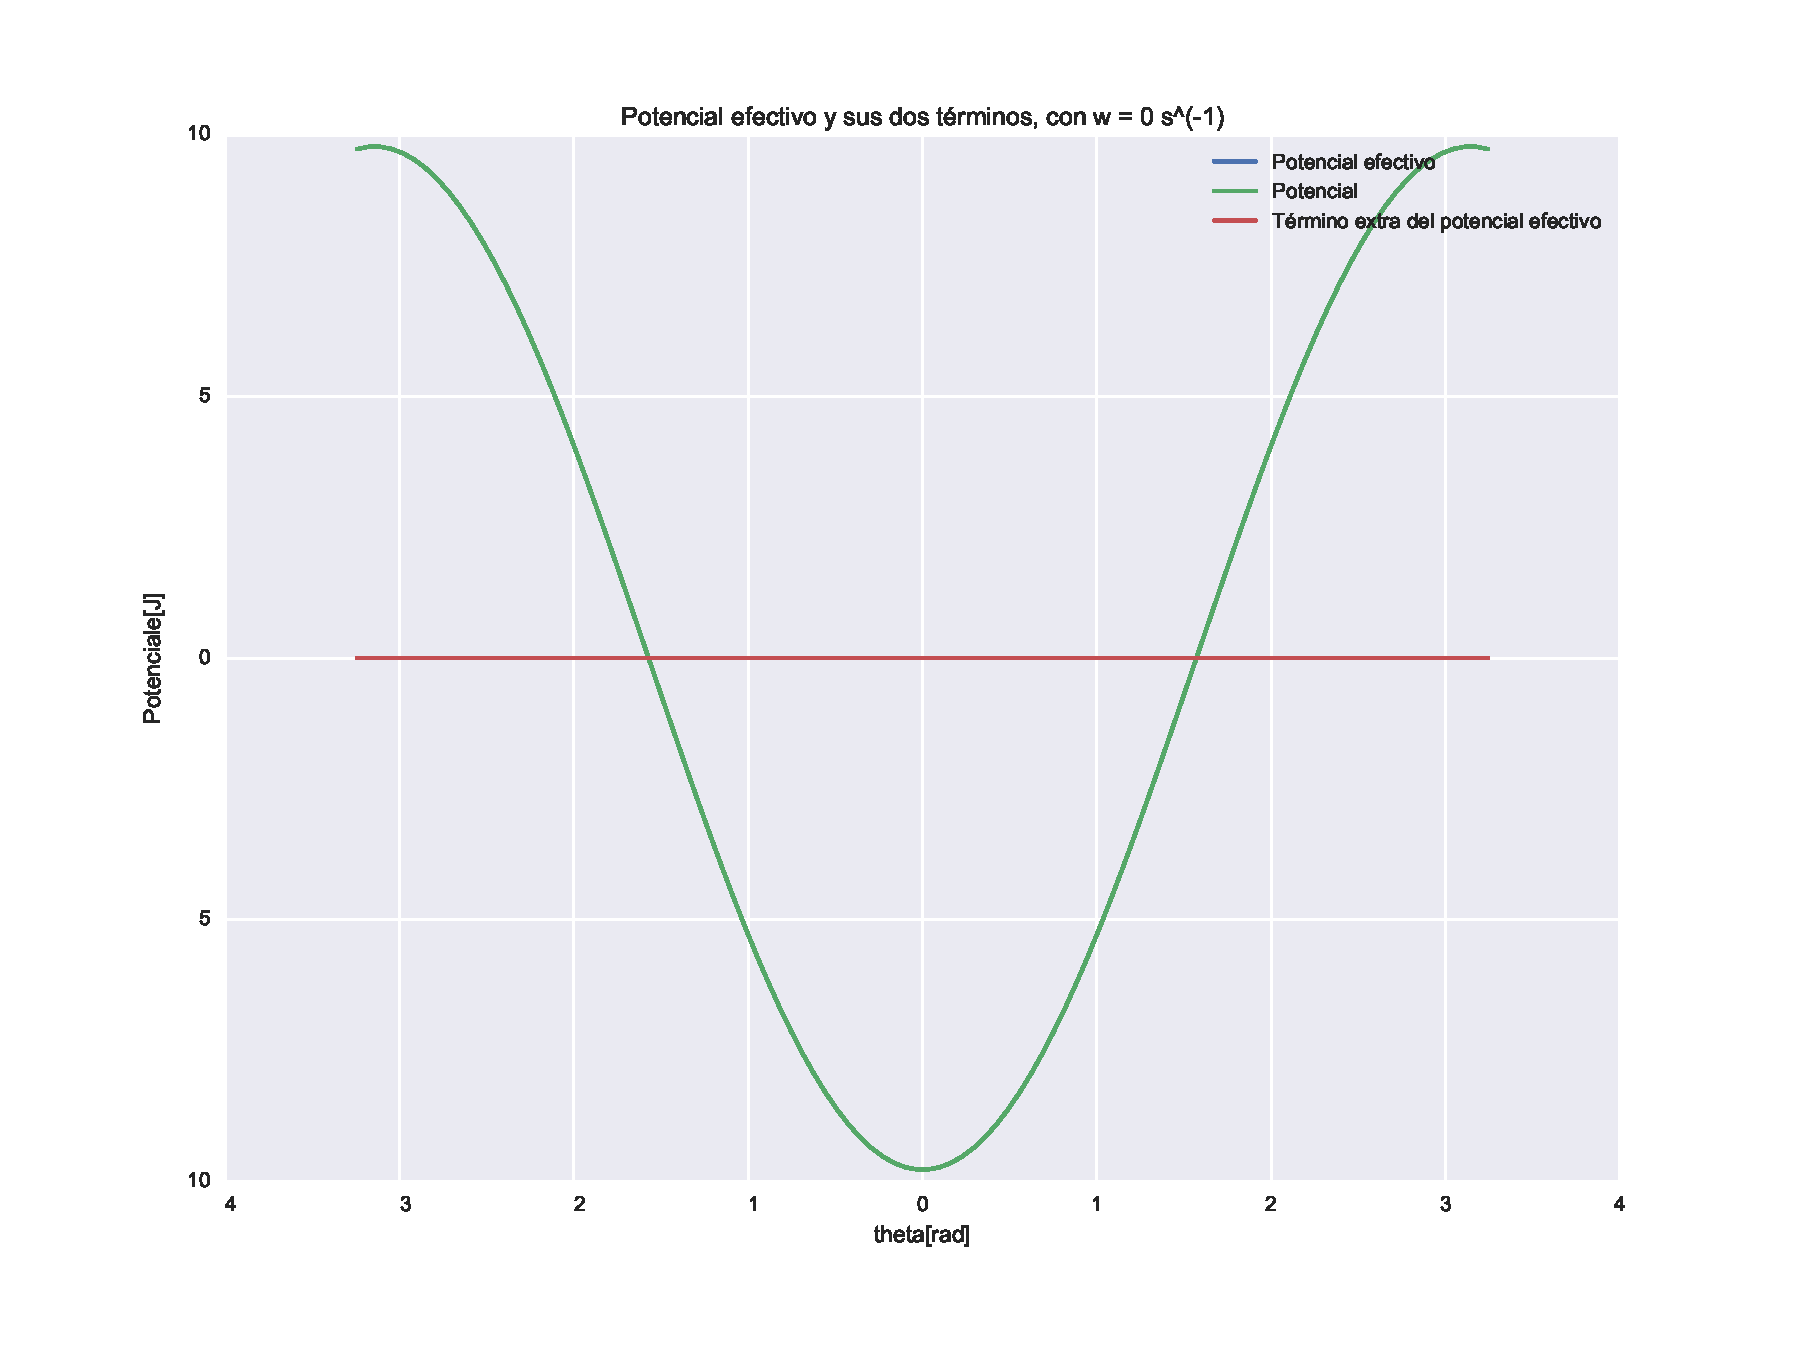
\includegraphics[width=0.7\textwidth]{w0.pdf}
\end{center}

\begin{center}
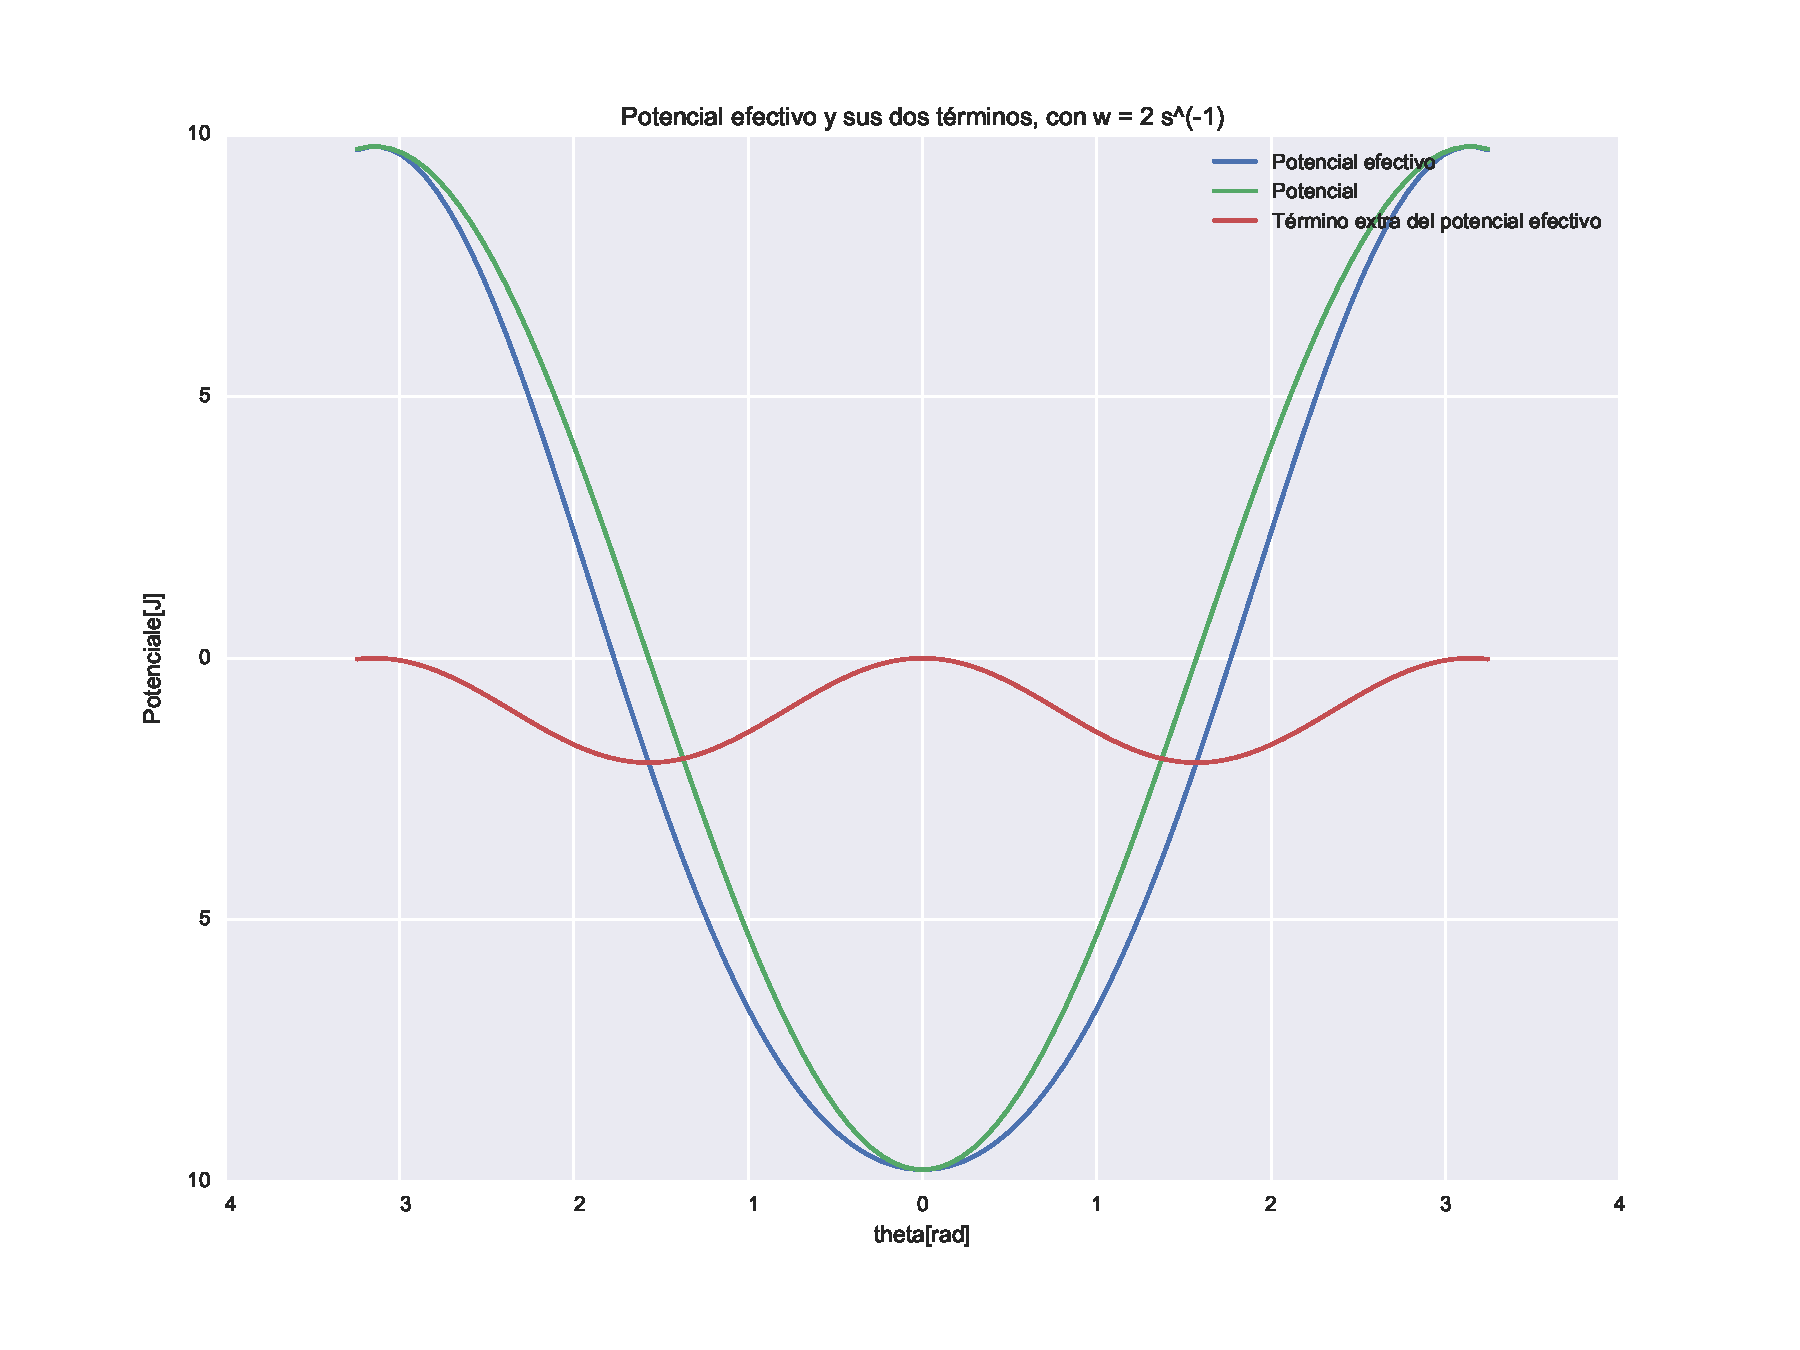
\includegraphics[width=0.7\textwidth]{wchico.pdf}
\end{center}

\begin{center}
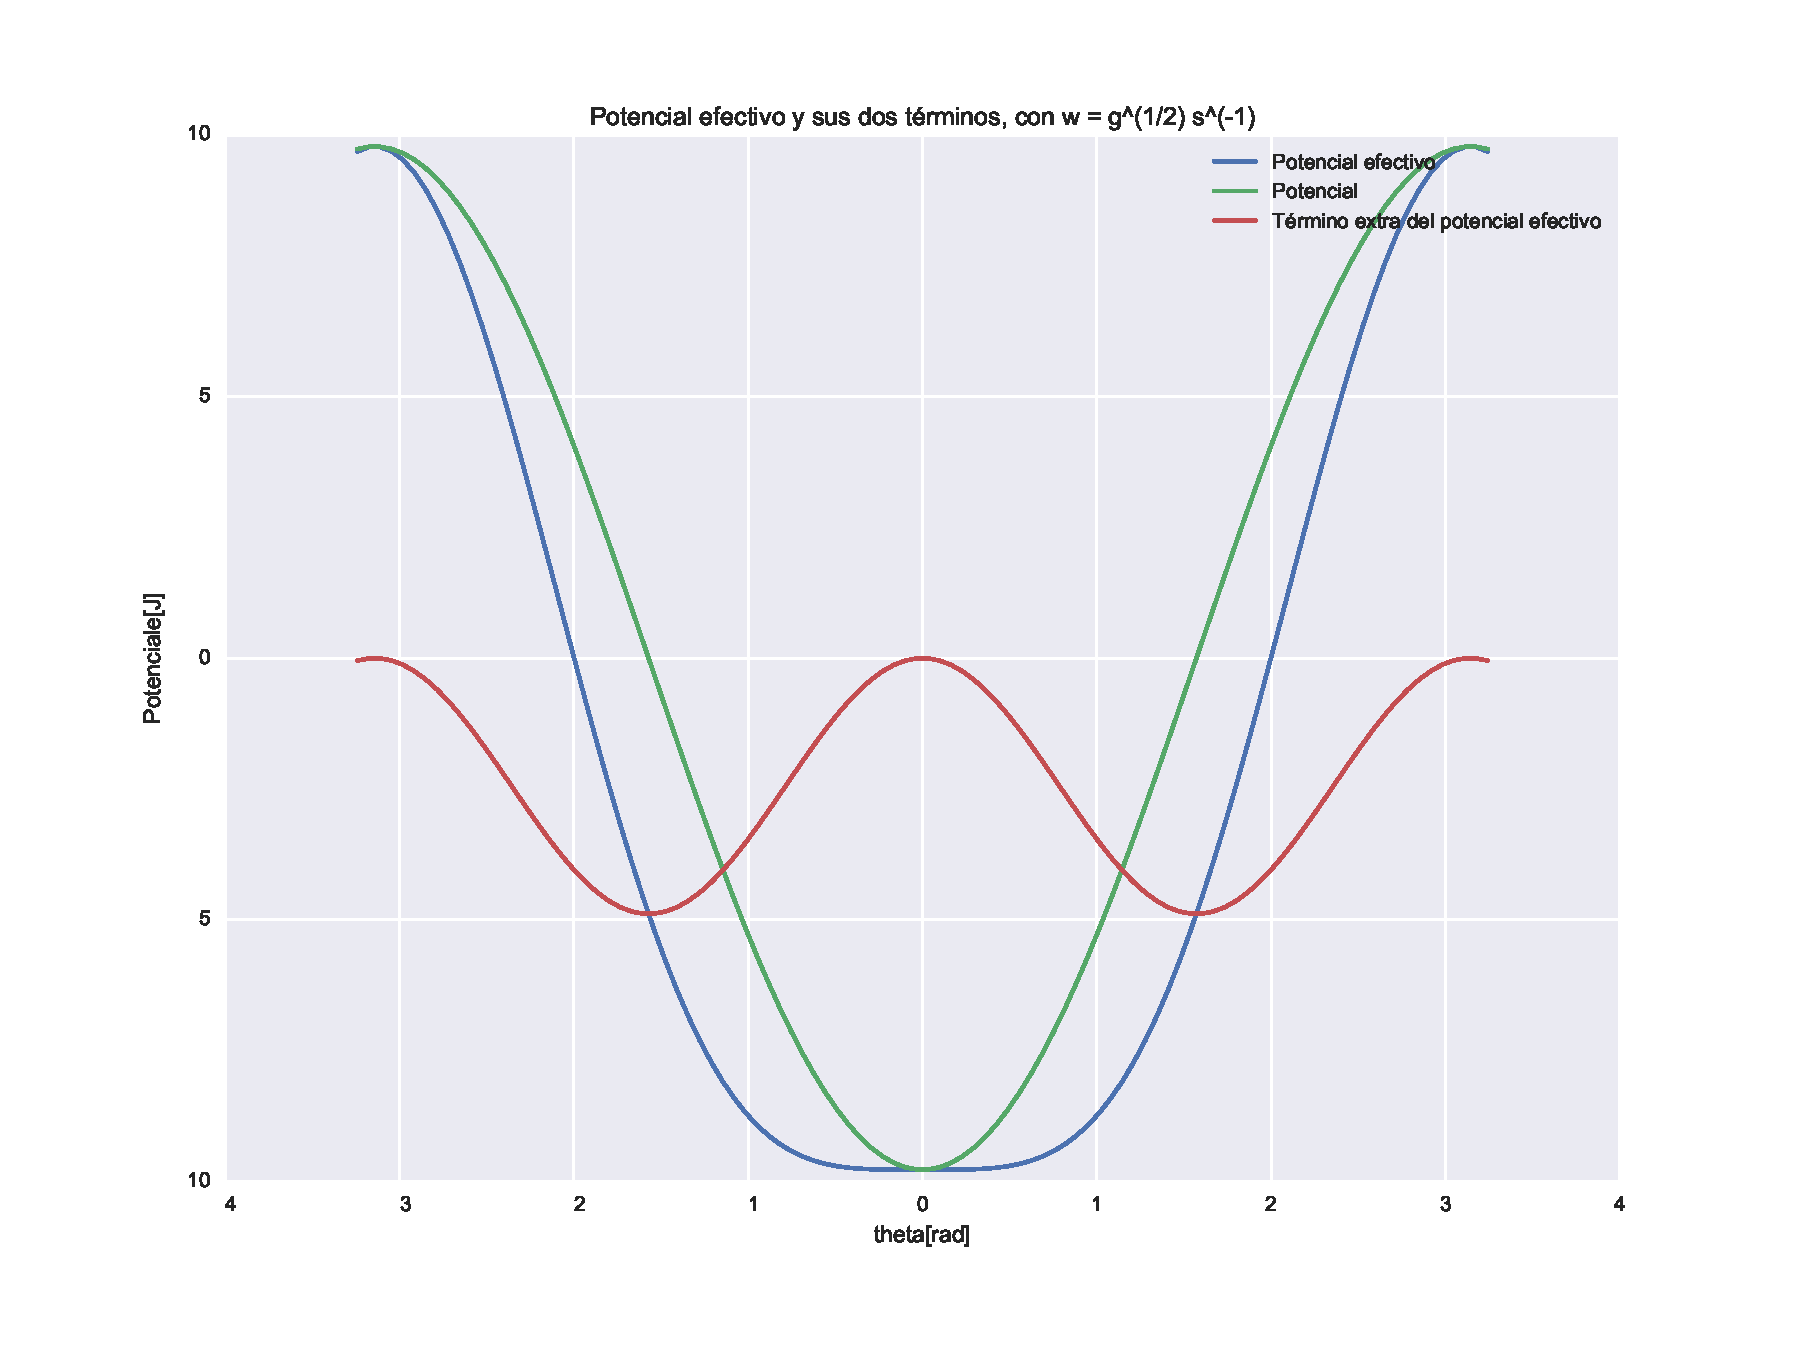
\includegraphics[width=0.7\textwidth]{wcritico.pdf}
\end{center}

\begin{center}
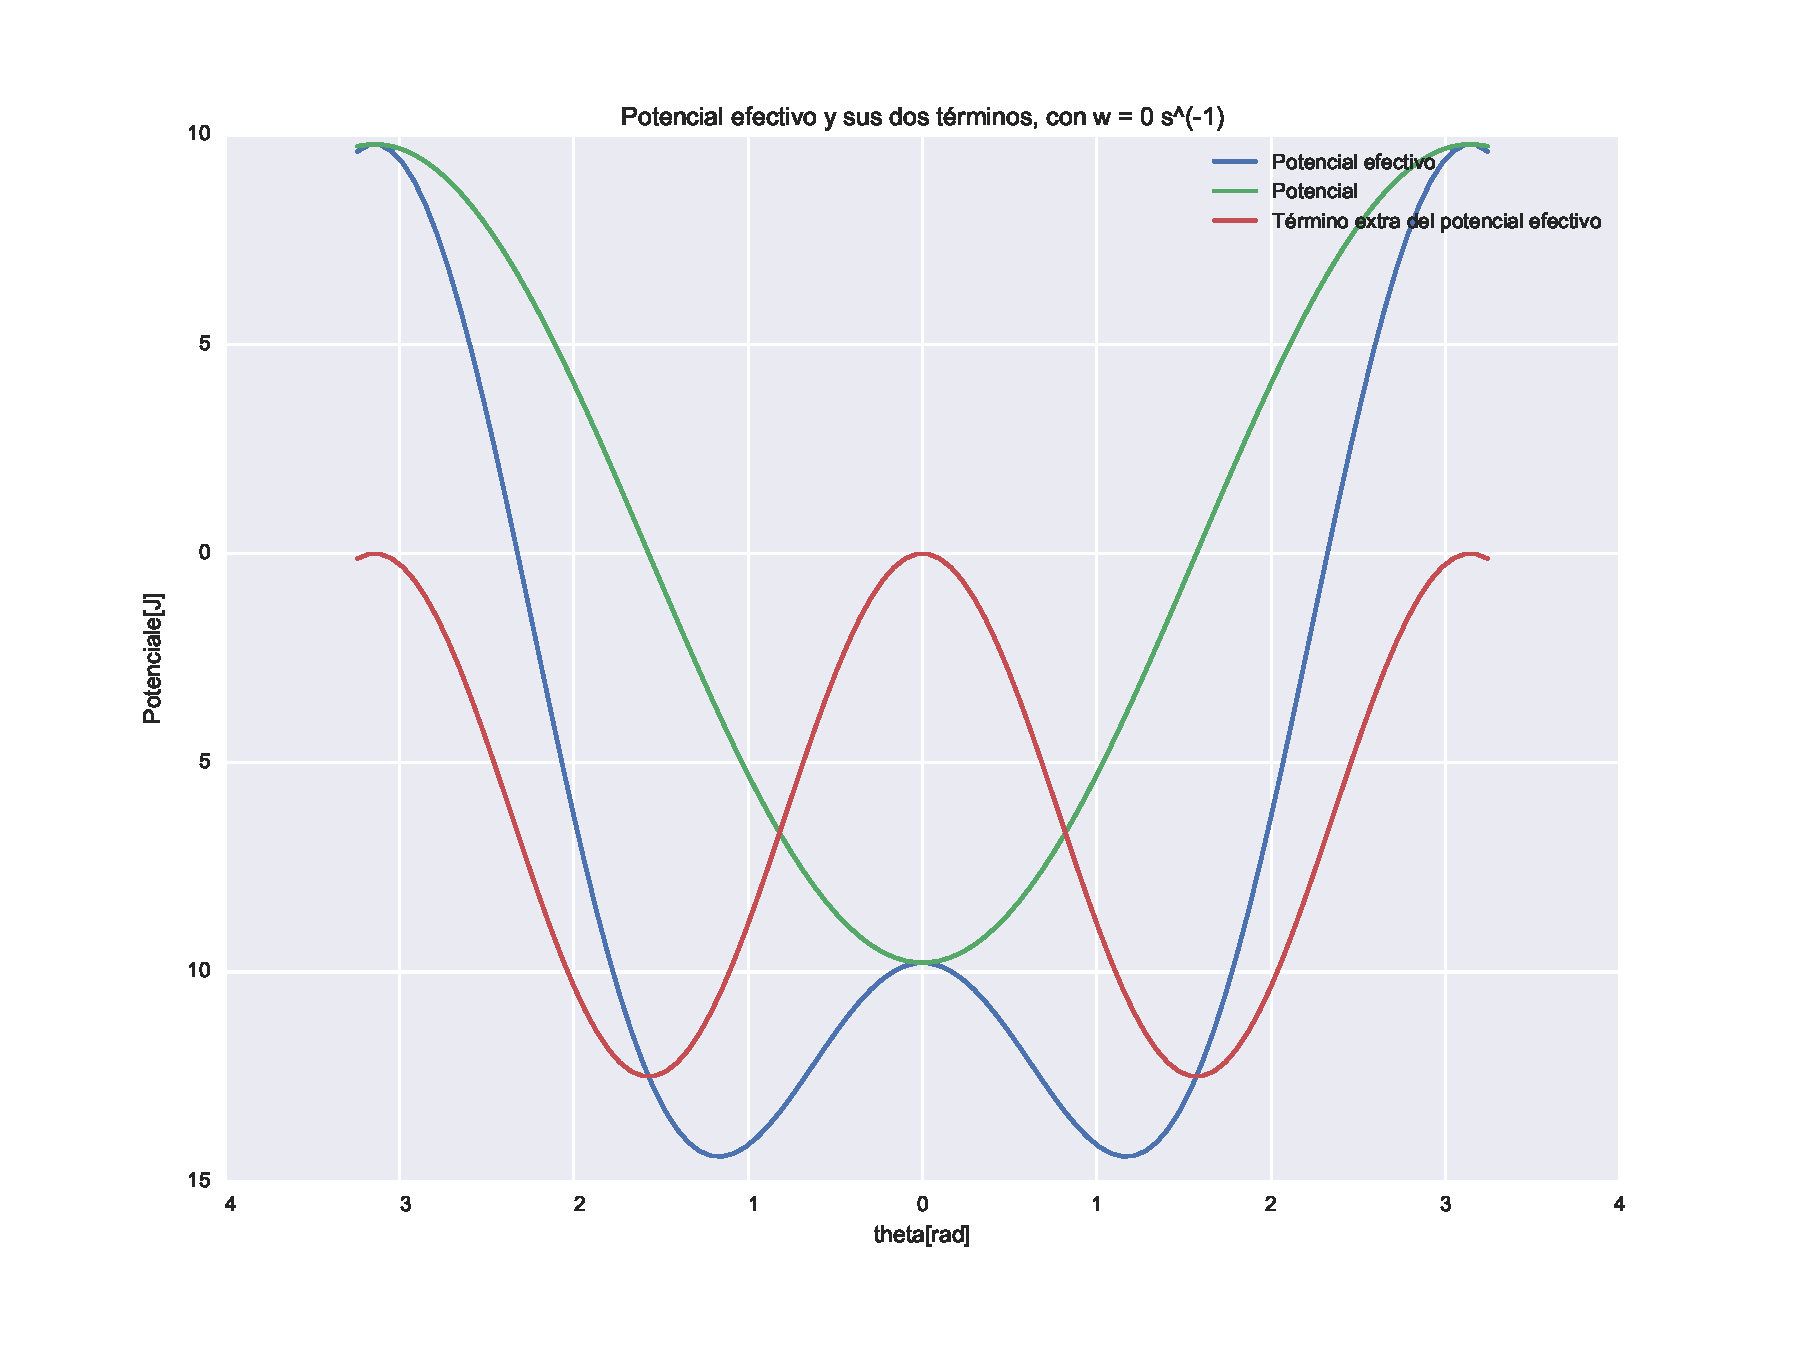
\includegraphics[width=0.7\textwidth]{wgrande.pdf}
\end{center}

\begin{center}
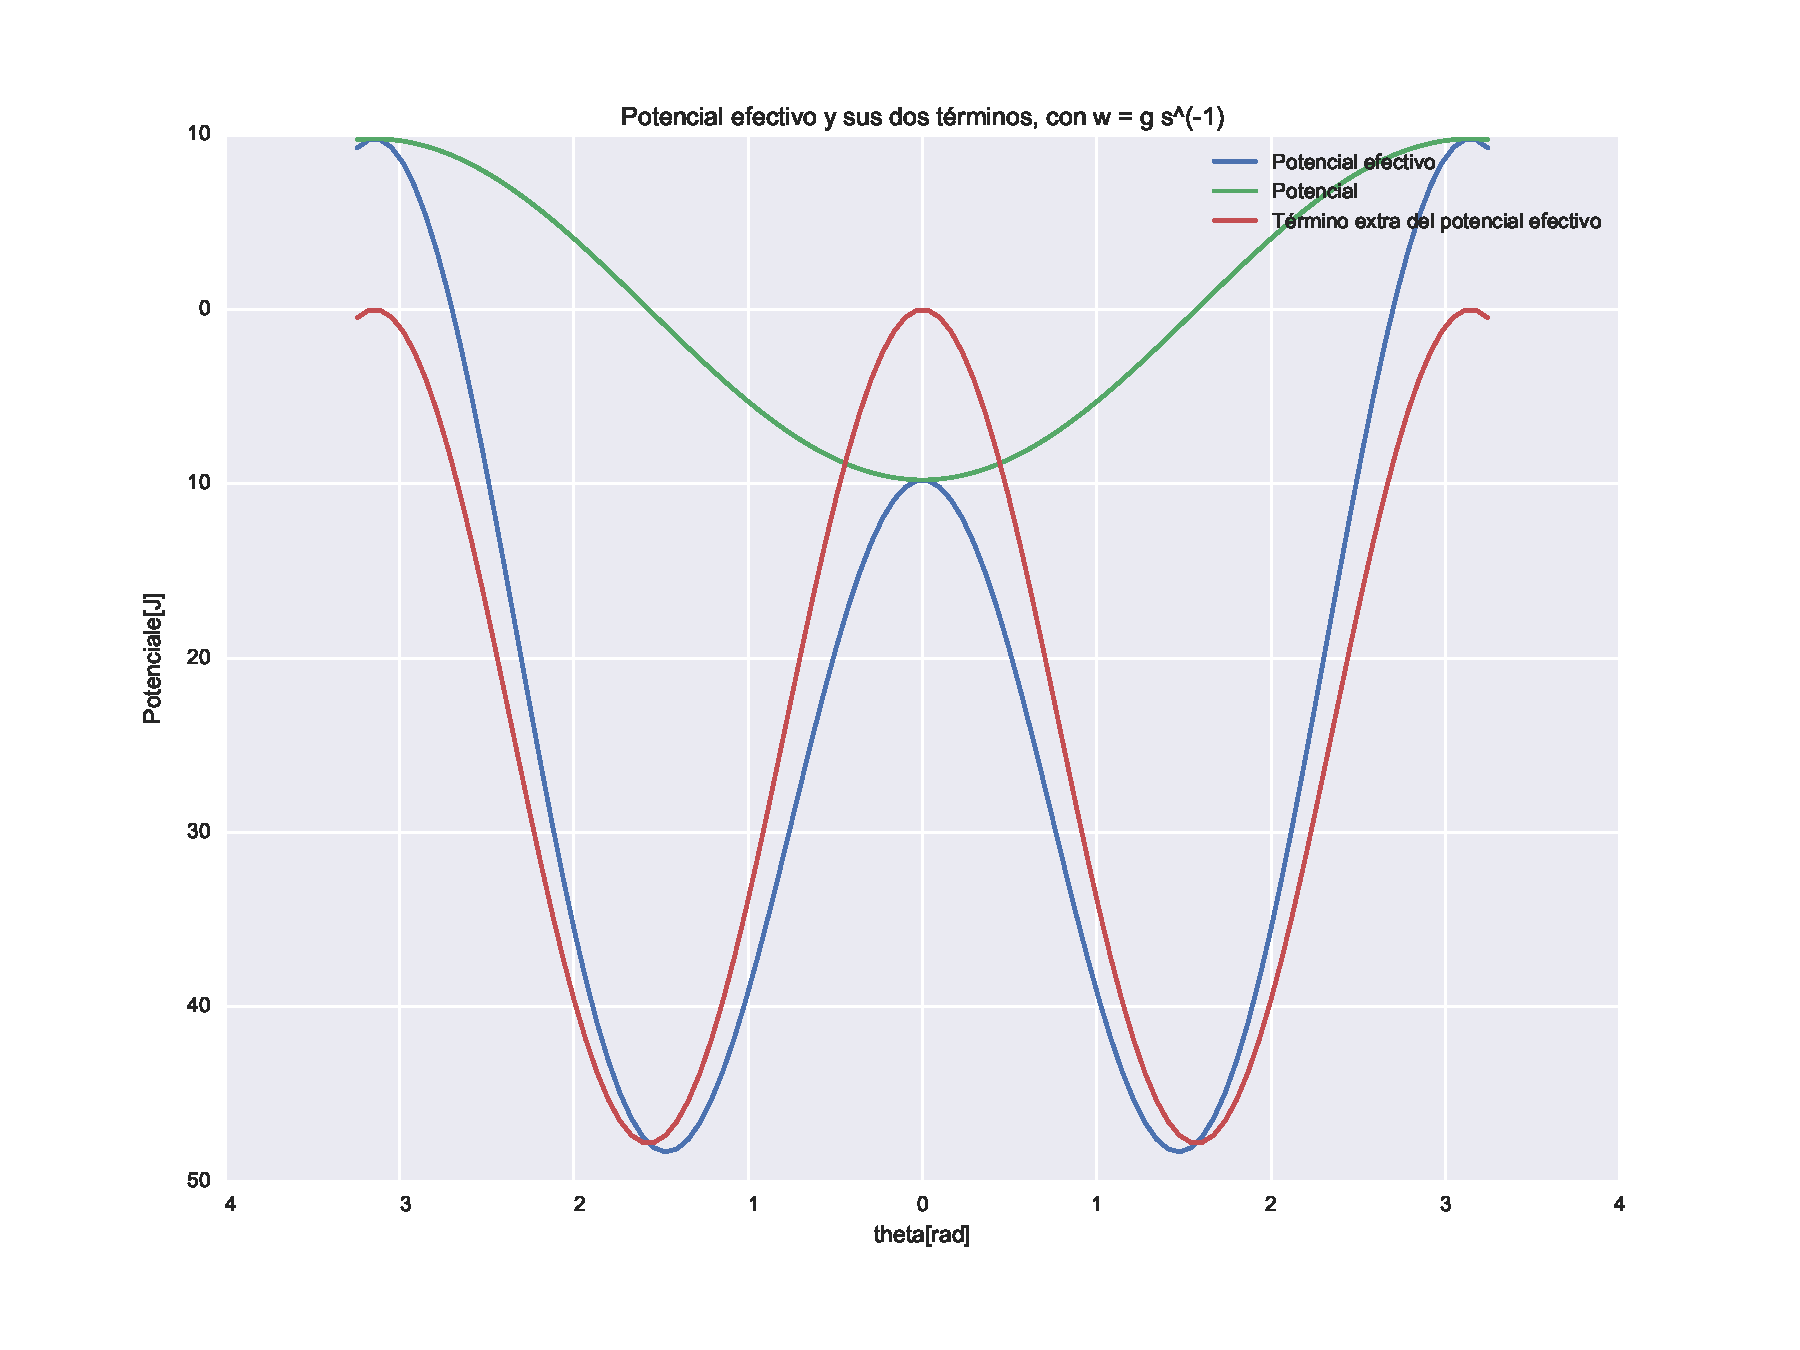
\includegraphics[width=0.7\textwidth]{wg.pdf}
\end{center}

\begin{center}
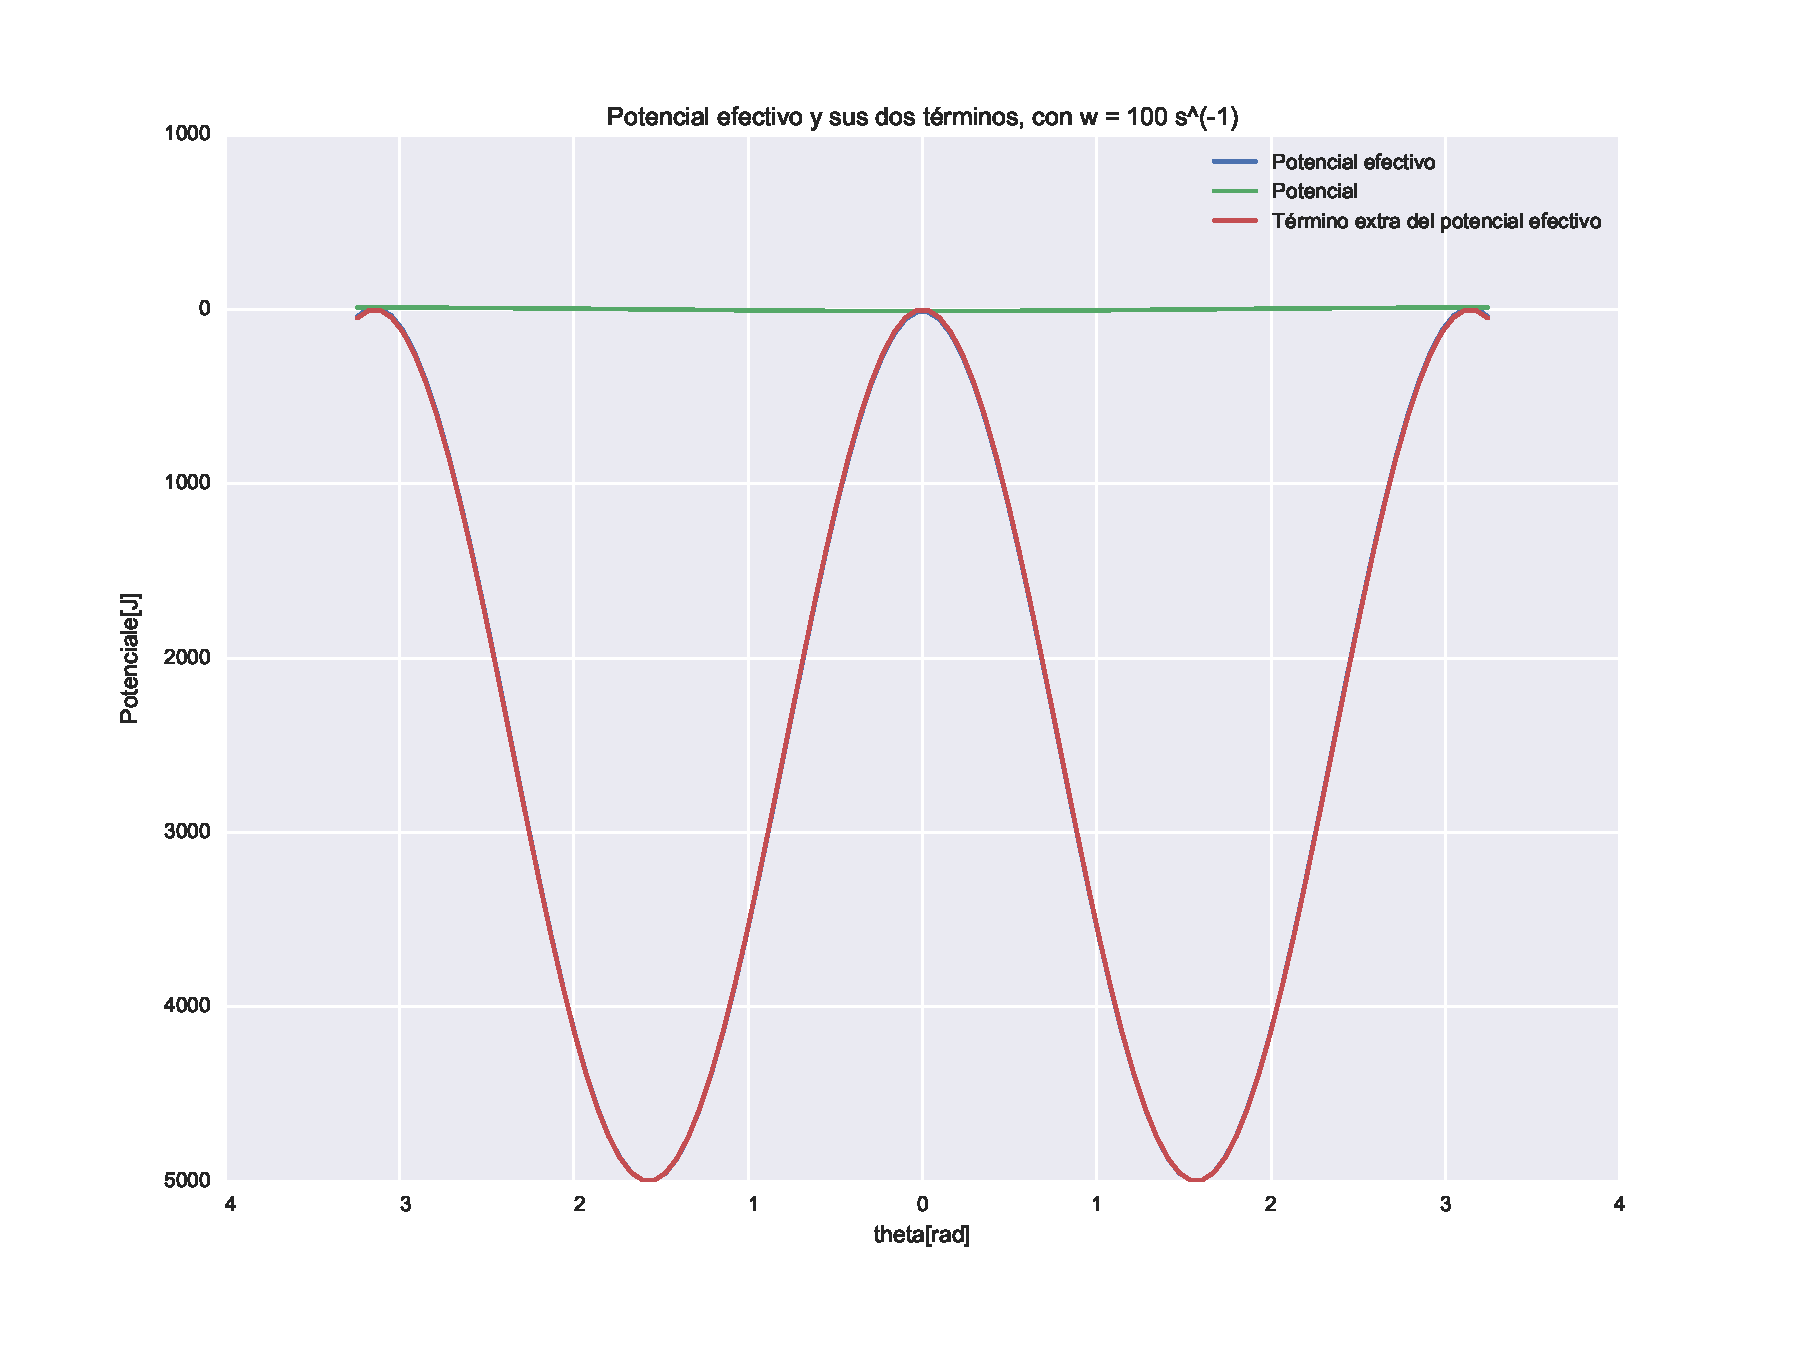
\includegraphics[width=0.7\textwidth]{wmuygrande.pdf}
\end{center}

\section{Materiales} 
\begin{itemize}
\item Tres aros de costura de diferentes di\'ametros. ($D_{1}= 24.5 cm \pm 0.05 cm$ $D_{2}= 26.5 cm \pm 0.05 cm$ $D_{3}= 30 cm \pm 0.05 cm$).
\item Circulos de pl\'astico transparente (2 por cada aro de costura, con el mismo di\'ametro que el aro).
\item Brushed motor de 9V conectado a un potenci\'ometro continuo de 9V.
\item Fotocompuertas marca PASCO, modelo ME-8932.
\item Pegamento Contactceys marca Ceys.
\item Duct Tape marca Tuk.
\item Canicas peque\~nas.
\item En el circuito:
	\begin{itemize}
	\item H-board.
	\item Cables para el circuito.
	\item Dos resistencias de $10 Kohm$.
	\item Potenciometro continuo de 9V
	\end{itemize}
\item Flex\'ometro.
\end{itemize}

\section{Metodología}
\noindent Primero, se monta el aro sobre el motor. Para esto se usa un CD como soporte. El aro se estabiliza fijandolo con una aguja o clavo en su parte posterior, sobre el eje de rotación. Esto se logra usando soportes universales. El motor está sostenido por un brazo para soldar electrónica. Para una mejor idea del montaje sería buena idea dar un vistazo a los videos. El motor está conectado a un circuito electrónico, que en escencia consiste de un Arduino, una H-Bridge, un potenciometro de $10 \mathrm{k\Omega}$ y una batería de $9 \mathrm{V}$. Esto nos permite controlar con precisión del motoro (que es un \emph{brushed} sencillo). Simultáneamente se monta la cámara (en este caso un \emph{Huawei P9 lite}) a la altura de el aro (ya sea la base o el punto medio, nosotros escogimos el segundo). El análisis se deberá hacer considerando esta posición. El montaje se hace en un tripié o soprte universal de piso. Se toma especial consideración, de que la cámara y el aro tengan la misma inclinación, preferencialmente ninguna. Finalmente, se preparan las fotocompuertas. En modo "péndulo'' se puede medir el periodo de osciliación al sujetar una tripa de plástico al cd y dejar que las fotocompuertas midan las interrupciones de la tripa. Hay que considerar que al medir en modo péndulo se mide dos veces el periodo de la rotación, es decir el valor real es la mitad del medido.
\par Ahora, comienza la experimentación. Primero se monta el aro de radio mayor (véase \emph{Material}), dentro de este se coloca una canica de masa $\mathrm{m_1}$. Las canicas se pesan anteriormente con una báscula. Ahora, se ajsuta el motor a una velocidad. Después de que el motor haya alcanzado este valor, se empieza a medir con las fotocompuertas y se empieza a rodar el video. Se toman 6 valores del periodo y 30 segundos de video. Así se tienen suficientes valores para tener significancia estadística (en partícular con el video se tienen c.a. 900 marcos). Después de esto se ajusta a otra velocidad y se repite el proceso. Una última vez, se repite el proceso.
Como las fotocompuertas estaban programadas para medir periodos de péndulos, los resultados obtenidos de T NO fueron periodos, sino el doble de un periodo. Así, la velocidad angular estuvo dada por:
$$w=\frac{4\pi}{T}$$
\par Ahora se desmonta el aro grande y se monta el aro pequeño, se ajsuta la cámara adecuadamente. Además se cambia la cánica de aro, asi encontrándose ahora en el ahora montado. Se repite el proceso de medición con tres velocidades distintas. Se desmonta el aro, se reemplaza por el aro de radio intermedio, ahi encontrandose la canica ahora y se toman tres mediciones con tres velocidades distintas.
\par Finalmente, se mantiene el aro de radio intermedio y se ajusta a una velocidad constante. Se toman mediciones ahora con la misma velocidad pero una mas $m_2$ que corresponde a otra canica y a una $m_1 +m_2$ donde se meten en el aro ambas canicas. El proceso de medición no cambia. Además, en todo momento se toma nota de si hubo movimiento o no de las canicas. Un análisis más profundo de esto movimiento no será posible sin una cámara que permita grabar rotando (tampoco es el propósito de el experimento).

La obtención de datos en Tracker tuvo que tener una metodología muy cuidadosa, ya había muchos factores que podían cambiar los resultados completamente. Para empezar, todo el análisis fue realizado exclusivamente en intervalos de tiempo de un medio periodo (a excepción del 2do video, el de R(14.2cm) y w(4.7098rad/s)). Es decir, todas las mediciones en el video fueron realizadas en los momentos en los que el aro estaba lo más alineado paralelamente a la cámara, ignorando las imágenes intermedias, para eliminar errores de perspectiva. Se optó por intervalos de tiempo uniformes para poder tener un mejor análizis del comportamiento de la canica, ya que con intervalos irregulares un presunto comportamiento simétrico no podría ser detectable. Es obvio que al querer medir cada media vuelta muchas veces no hubieran alineaciones perfectas, creando un error de perspectiva, pero éste fue ignorado, ya que no era comparable con el error dado por el tamaño de la canica. Ésto es completamente justificable, ya que en las imágenes en las que había una alineación satisfactoria, si uno avanzaba a la siguiente imágen, el cambio de la posición del centro de la canica nunca fue mayor a su radio.

El siguiente factor en cuestión fue el posicionamiento del origen de coordenadas. Es lógico que si uno mide la posición del centro de la canica, entonces su movimiento tomará lugar en una circunferencia de menor radio que la del aro, por lo que el origen de coordenadas no debe estar en la base del aro. Así, con vectores en Tracker se midió el radio de los dos tipos de canicas usadas y respectivamente se usó para poder ubicar el origen de coordenadas. Por otra parte, basta con ver un par de videos y una toma de datos a ciegas para poder darse cuenta de que la cámara no estaba perfectamente con el eje de giro, por lo que, debido a que las mediciones se tomaban cada media vuelta, poner el eje de coordenadas derecho provocaba que las mediciones alternaran. Es decir, las mediciones de un lado del eje podían ser más grandes que las del otro lado (tomando en cuenta la altura). Ésto provocaba que la desvicación estándar de la altura se duplicara y que se perdiera mucha exactitud. Así, para alinear los ejes se tomaron en cuenta dos puntos de los cuales estábamos seguros que estuvieran fijos: el punto de contacto del motor con el aro y el punto de contacto del tornillo con el aro. Después de eso, solo bastaba con tantear los ángulos de inclinación del sistema de referencia en tracker para que el eje estuviera alineado con el motor y el tornillo. Claro que el modelo asume que el eje de giro coincida con la dirección de la fuerza de gravedad, pero el efecto de ese cambio es despreciable, pues la corrección más grande que se hizo fue de 2 grados.

Por último, todas estas correcciones invalidaban el uso del radio medido del aro como parámetro del modelo, por lo que se prosiguió de la siguiente manera: Se creó un vector paralelo al eje de giro (por lo que se tomó como guía el eje vertical del sistema coordenado), que va desde el origen hasta la parte superior del aro. Se calculó su magnitud y a élla se le restó el radio de la canica y se dividió entre 2. El resultado sería la magnitud del vector que va desde el origen hasta el centro de la circunferencia en la que sucedía el movimiento (ésta magnitud aún no se toma como el radio, ya que los aros no eran perfectamente circulares y en cada caso se debía tomar en cuenta el diferente radio, que dependía de la altura de la canica en el aro). Éste procedimiento se puede ver en la siguiente imagen:

 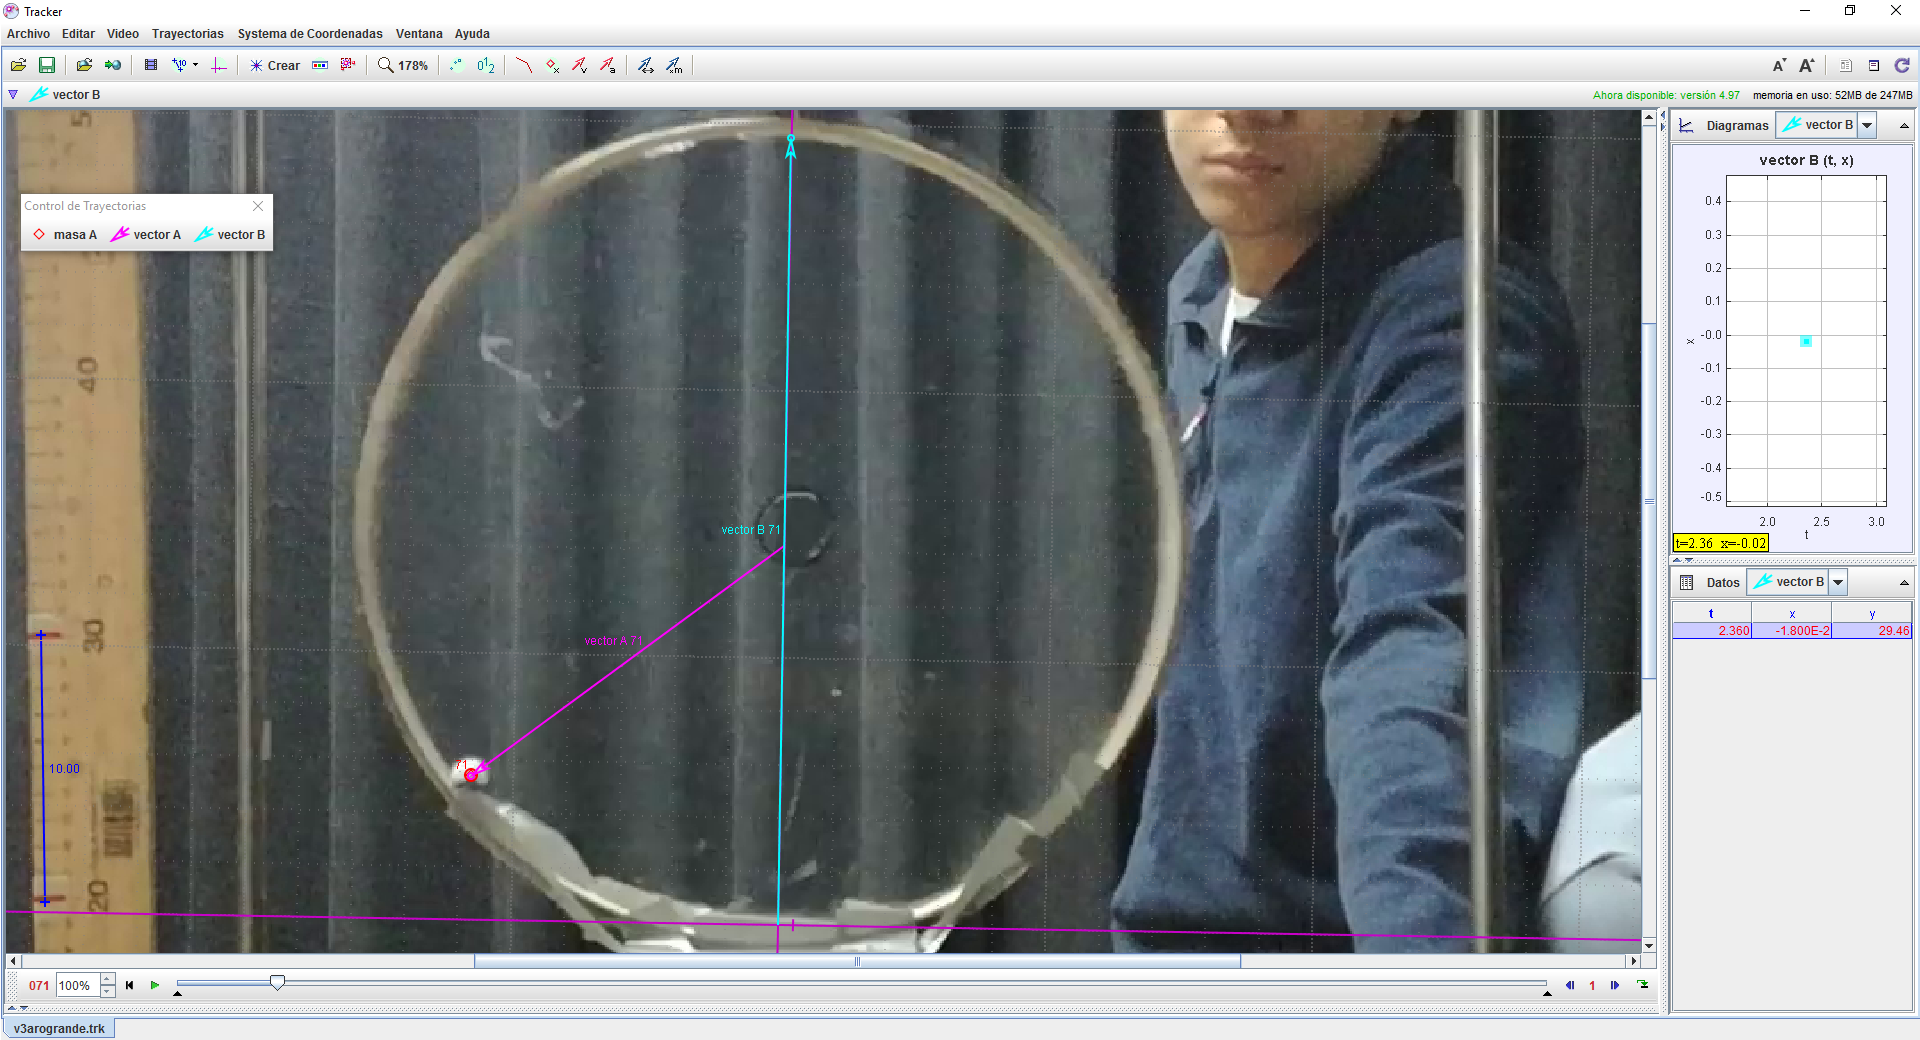
\includegraphics[scale=0.37,center]{aro1}

Ubicando el centro de dicha circunferencia mediante otro vector de dicha magnitud, se dibujaba otro vector que iba desde el centro de la circunferencia hasta al centro de la canica. Así, la magnitud de éste vector fue la que fue tomada como radio de la circunferencia. Ésto se puede observar en la siguiente imagen:

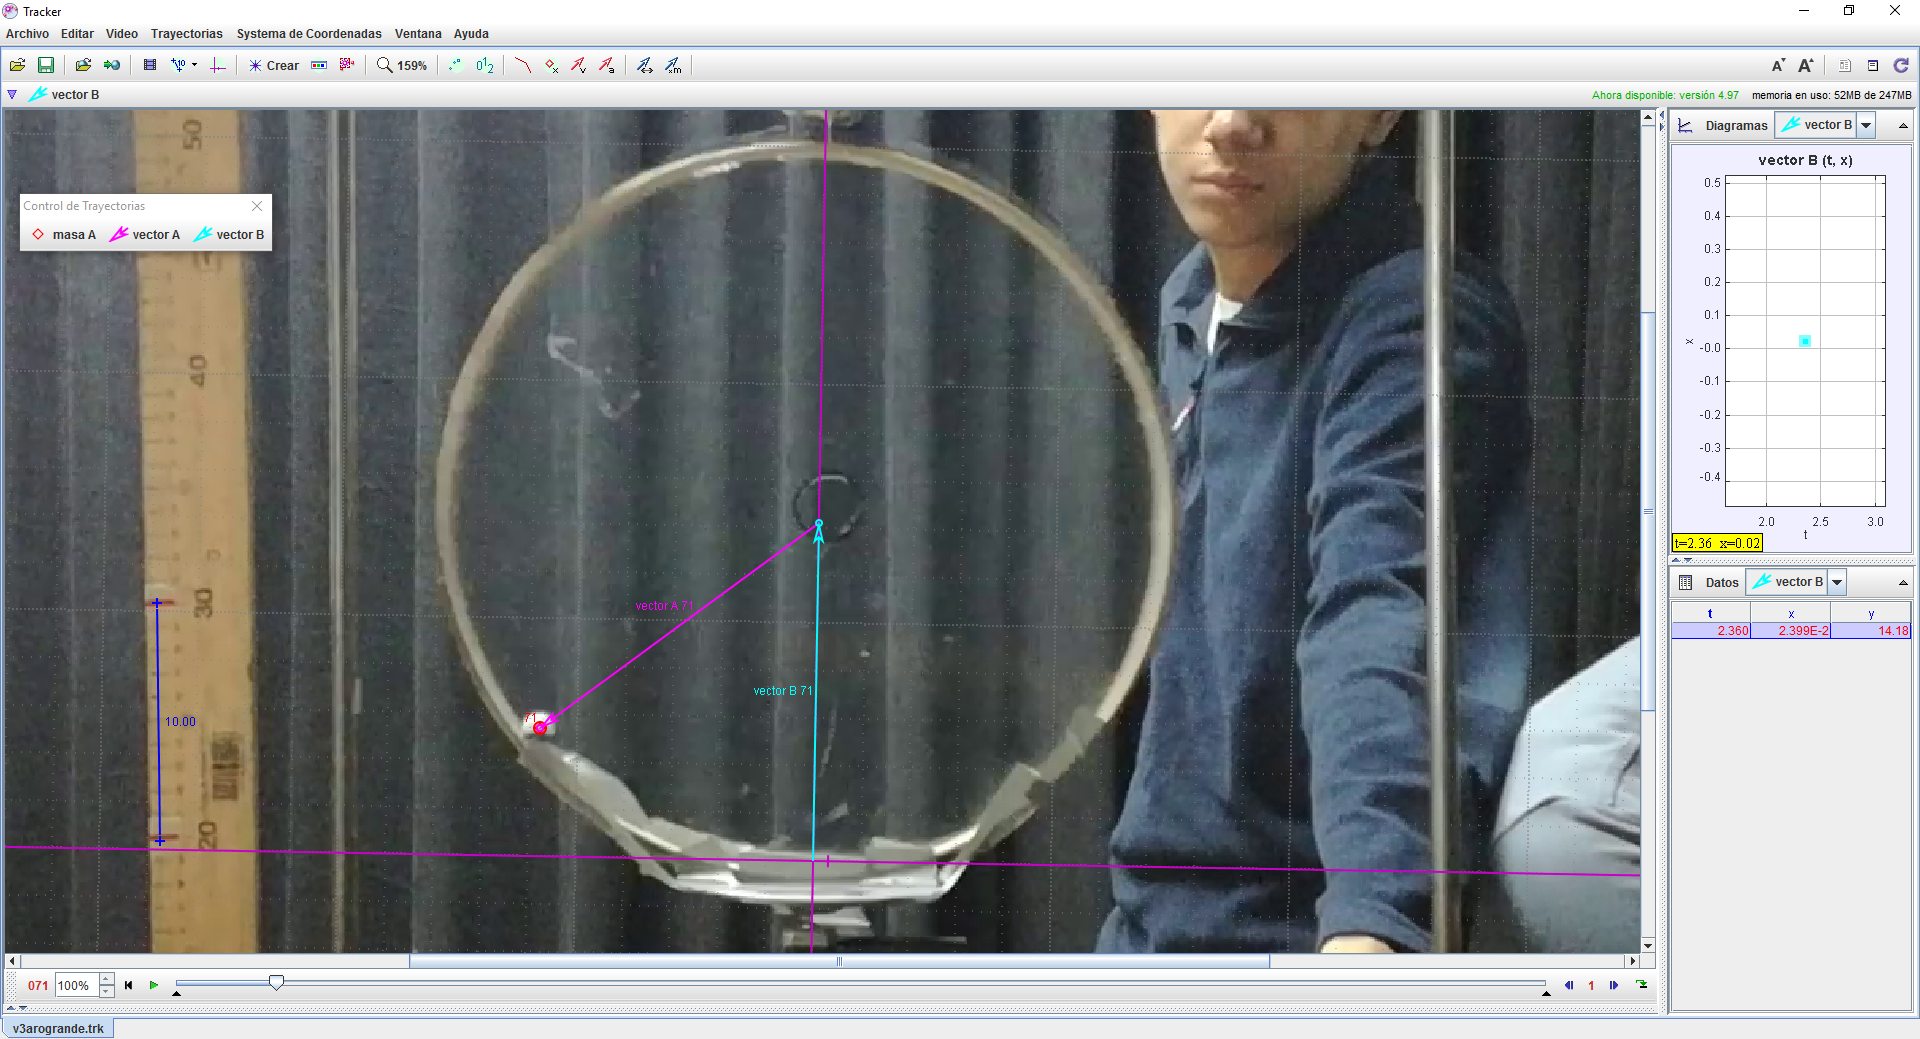
\includegraphics[scale=0.37,center]{aro2}

 Éste procedimiento fue realizado en la primera imagen que fue tomada en cuenta para cada uno de los videos, dejando así radios distintos para mediciones con aros iguales. Afortunadamente las diferencias no fueron muy grandes (la mayor diferencia entre radios de un mismo aro fue de 0.4cm), lo que denota que la deformación de los aros no fue muy grande, y todavía pueden ser considerados como circunferencias para efectos del modelo.

\par Para obtener datos de los videos  y para el análisis en sí se usa \emph{Python} y la paquetería para graficación y análisis de datos que lo acompaña. No se usan métodos estadísticos especiales.

\subsection{Determinación de incertidumbres}

Debido a que el radio de las canicas era considerablemente mayor a los pixeles por imagen, en las mediciones de distancias (tanto de la altura, como de la magnitud de vectores) el error asociado fue el del radio de la canica utilizada (que no fue la misma que la mencionada en la primera entrega, se utilizaron canicas del laboratorio), que fue medida con Tracker. La canica de $3.5g \pm 0.05g$ tuvo un radio de $0.7cm \pm 0.12cm$ (el error de la medición del radio fue el de la calidad de la cámara), la canica de $3.7g \pm 0.05g$ tuvo un radio de $0.8cm \pm 0.12cm$. Para cuando se utilizaron dos canicas se utilizó de igual manera el radio de $0.8cm$, ya que tomó la medición en el punto de contacto entre las canicas, por lo que, mientras que hoizontalmente el error se duplicaba, verticalmente no había un cambio apreciable.

Como las fotocomupertas nos dieron resultados de periodos con una presición de 4 cifras decimales, su valor es expuesto con ellas. Como el periodo utilizado fue el promedio de un conjunto de mediciones, su error asociado fue la desviación estándar de la muestra.

El error asociado a la velocidad angular, en términos de la T medida y su desviación estándar dT, obtenido mediante el método de fracciones parciales es:

$$dw=\frac{4\pi}{T^2}dT$$

El valor de la gravedad para la ciudad de méxico fue obtenido de una página web (ver ref. 1) que calculaba la aceleración de la gravedad local en base a la ecuación recomendada por el Boletín OIML - Número 127, junio/1992, con una exactitud del 0.01\%. Como el valor de la gravedad obtenido fue de $978cm/s^2$, su error asociado fue de $9cm/s^2$.

Como se verá a continuación, el error de las alturas medidas fue la desviación estándar de la muestra obtenida, ya que se realizaron múltiples mediciones de alturas por experimento. Por otra parte, el error de las alturas esperadas fue obtenido mediante el método de fraciones parciales aplicado al modelo, con los errores de los parámetros que lo definen. Así, el error de las alturas esperadas estuvo dado por:

$$dh^2=dR^2+\frac{dg^2}{w^4}+\frac{4g^2dw^2}{w^6}$$

Otro parámetro tomado en cuenta fue el de la velocidad angular crítica de cada circunferencia, que determina el valor mínimo para el cual la elevación de la canica va a ser mayor que cero. Como está dado por $\sqrt{\frac{g}{R}}$, su error asociado fue:

$$dw^2=\frac{dg^2}{4gR}+\frac{gdR^2}{4R^3}$$

\section{Resultados}
A continuación se muestran las gráficas y las tablas de datos de la altura de la canica con respecto al tiempo. Los puntos azules son los datos obtenidos. Se tomaron muestras de diferentes tamaños tomando en cuenta la desviación estándar. Es decir, entre mayor variación, se tomaban muestras más grandes. Como fue mencionado anteriormente, los intervalos de tiempo son de medio periodo.
 El error de cada medición es el radio de la canica, por lo que se podría pensar que en las gráficas las barras de error de la altura representan la dimensión de la canica.
Como la altura máxima es constante en el tiempo, én este caso no hubo ajuste a mínimos cuadrados, ya que el modelo es simplemente un número (representado como una linea verde, con error dado por el error de los parámetros del modelo representado como una barra verde). Así, el resultado de cada conjunto de datos se tomó como el promedio de las mediciones, con el error asociado a la desviación estándar, representados como una linea roja y una barra roja, respectivamente.

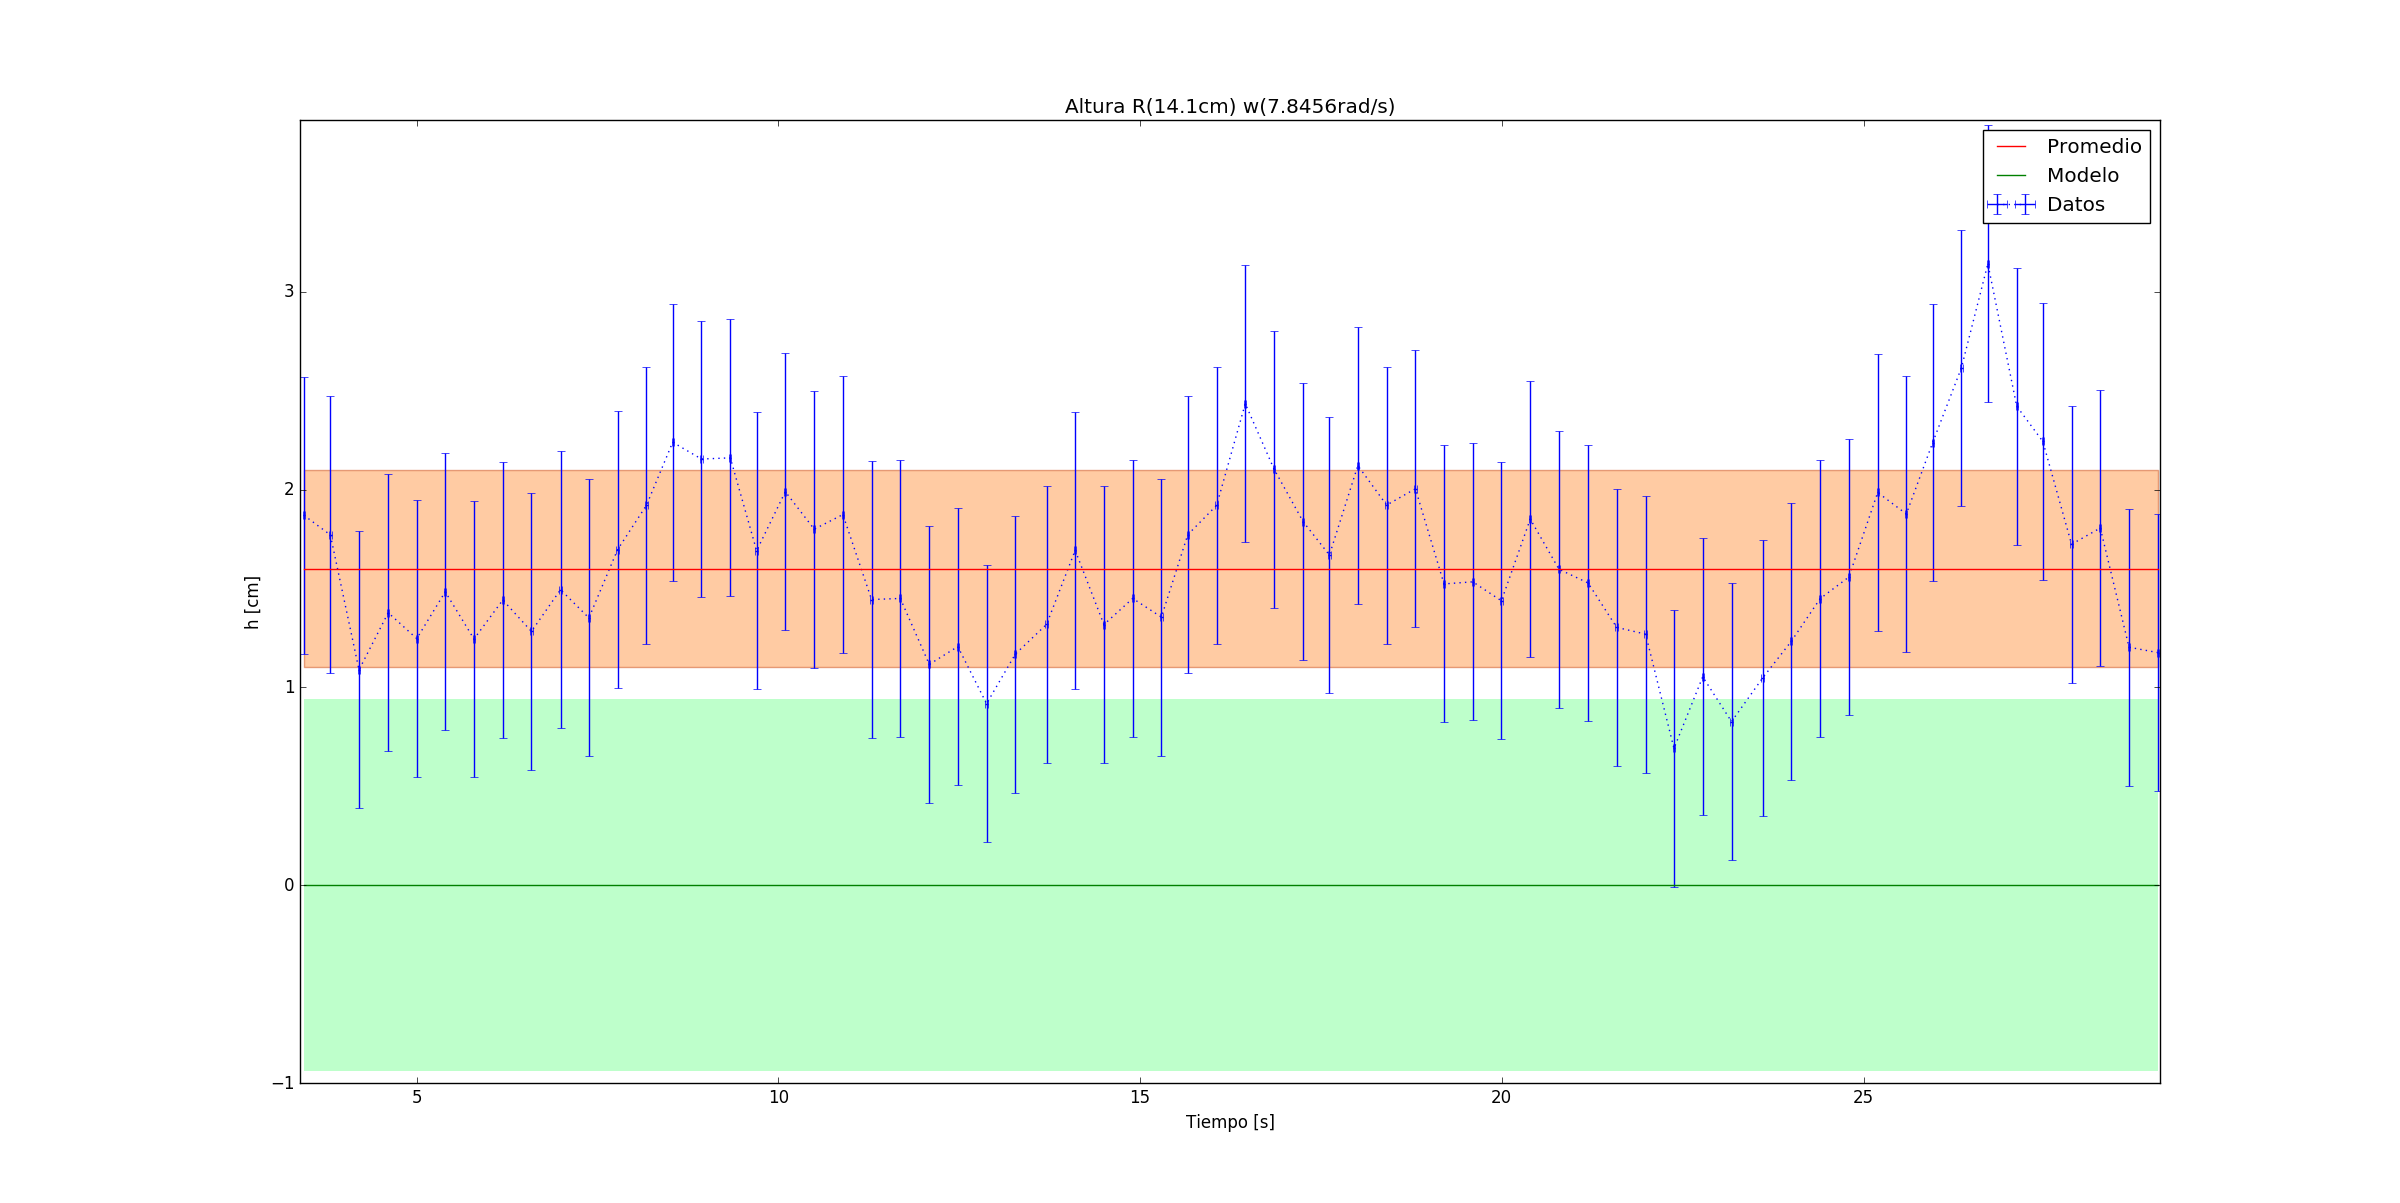
\includegraphics[scale=0.37,center]{1_1}
\begin{figure}
   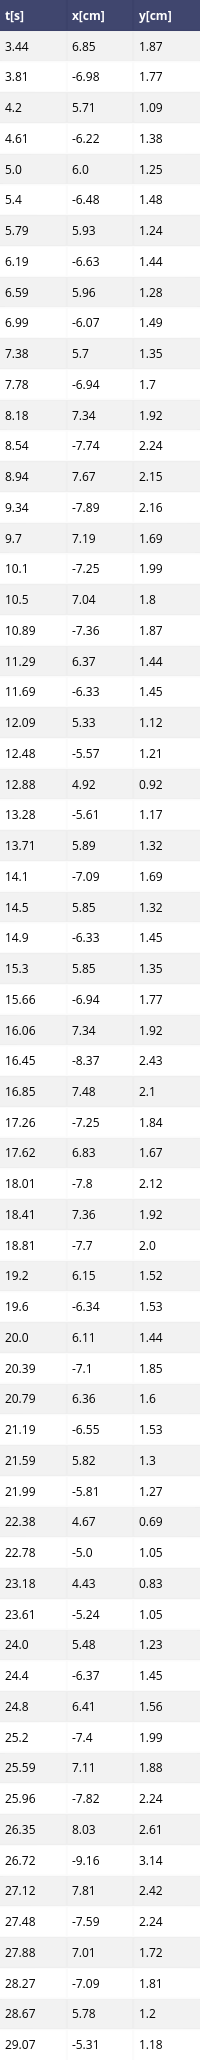
\includegraphics[scale=0.3,center]{t1_1}
  \caption{R(14.1cm) w(7.8456rad/s)}
\end{figure}

Las mediciones en R(14.2cm) w(4.7098rad/s) fueron las únicas que fueron realizadas en intervalos de tiempo dados por las fps de la cámara, ya que en éste caso la canica mantuvo un movimiento oscilante (lo cual era de esperar, pues para esa w, la canica debe tener el movimiento de un oscilador armónico para pequeñas variaciones de altura). Como se puede observar en la gráfica, hay huecos en el conjunto de datos que se deben a los momentos en los cuales el aro tapaba a la canica y no se podía hacer medición alguna. Todas las implicaciones de ésta medición serán abordadas en la discusión.

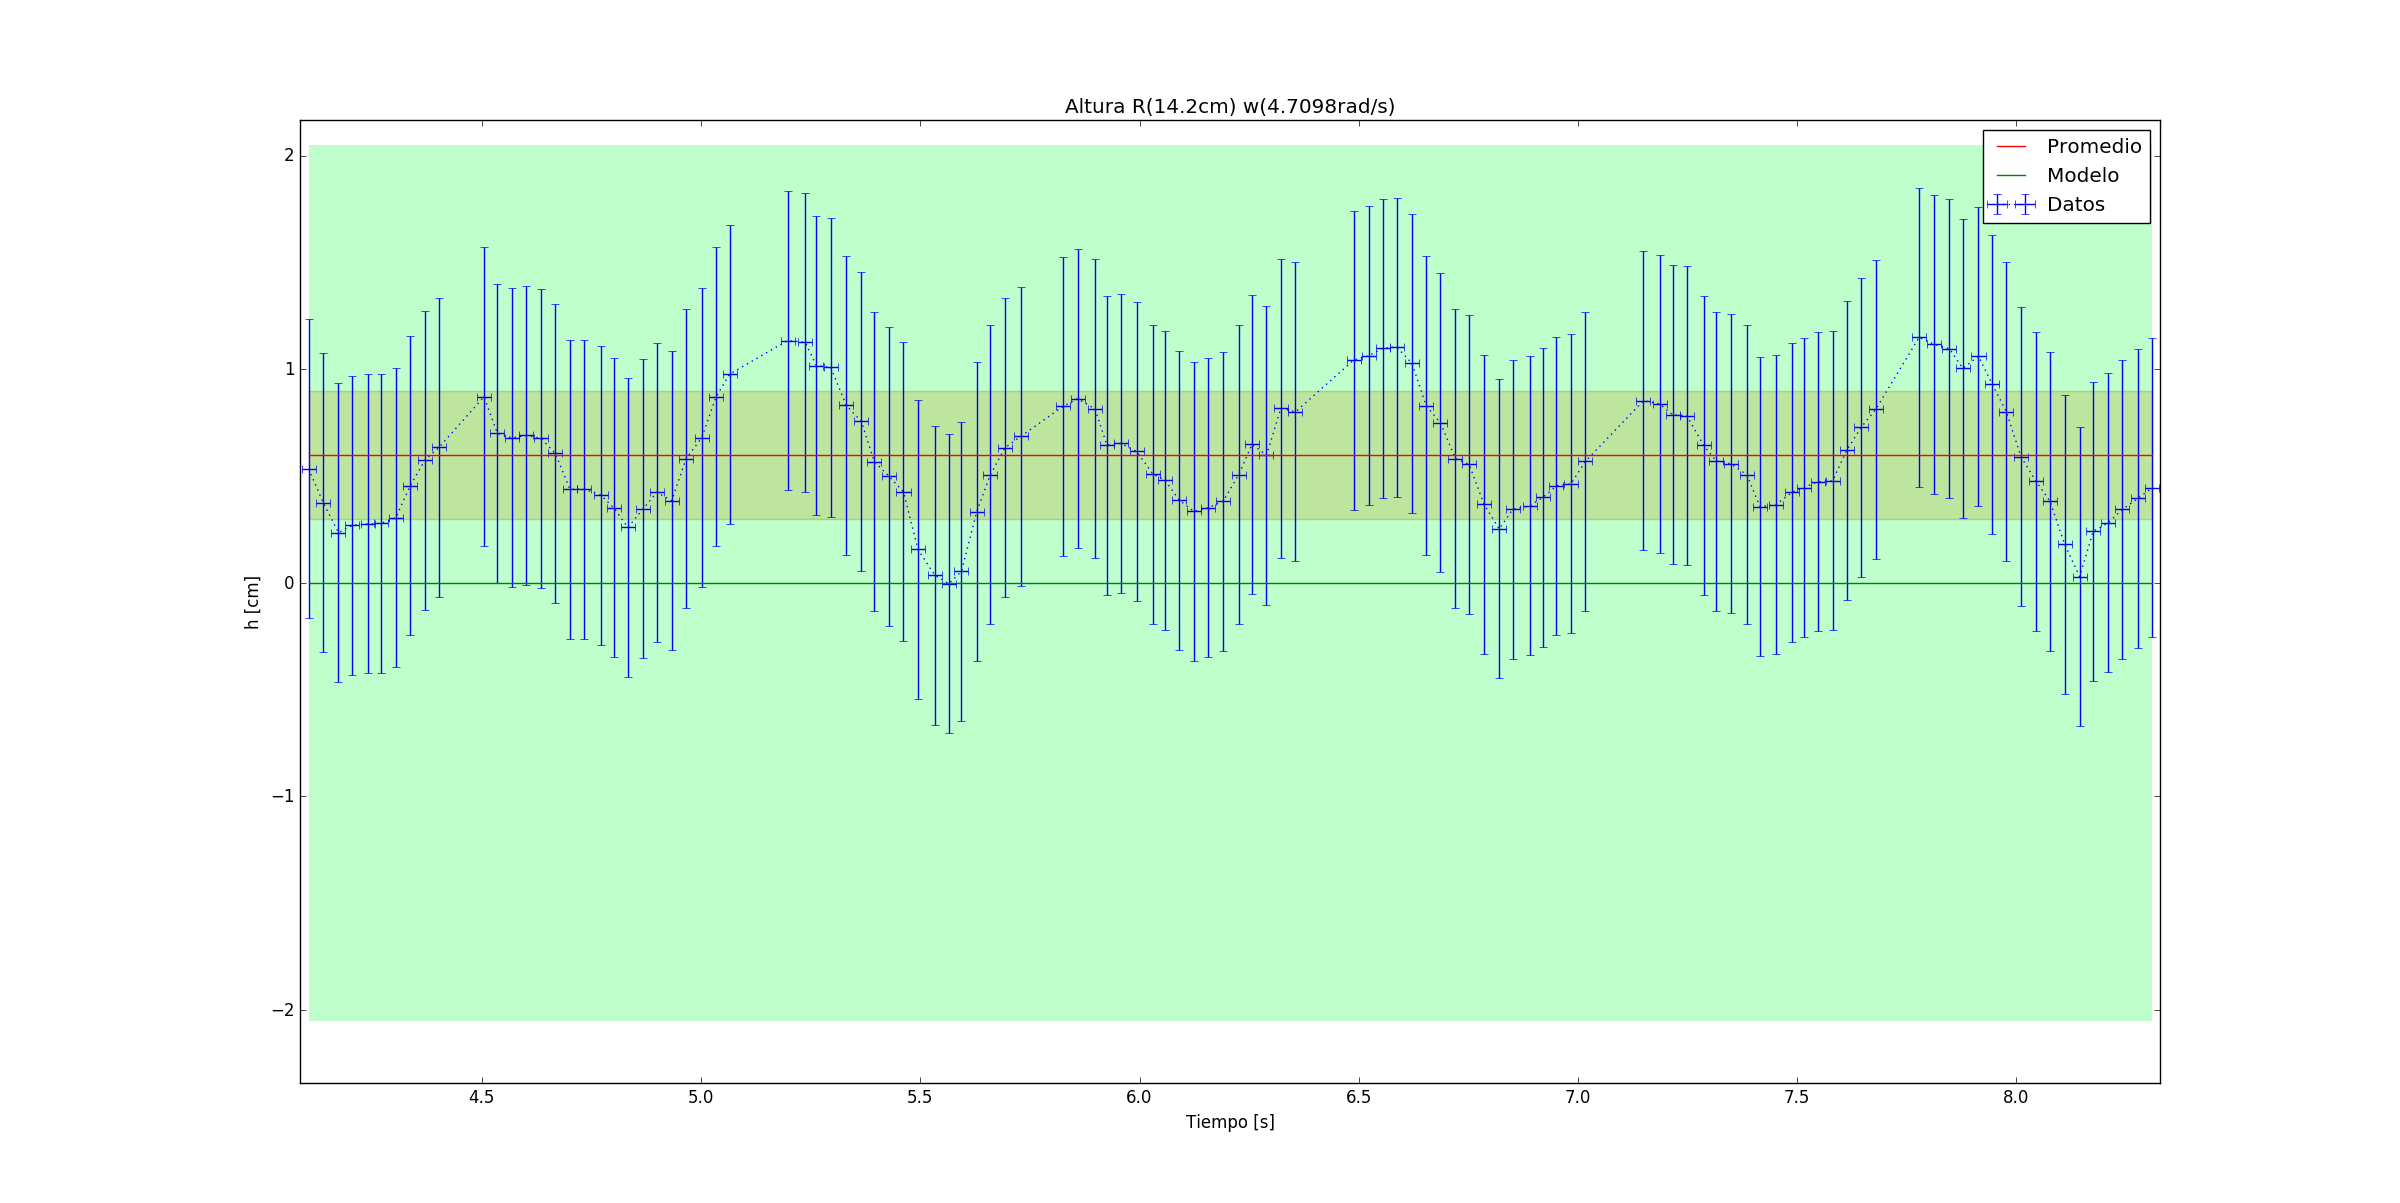
\includegraphics[scale=0.37,center]{1_2}
\begin{figure}
	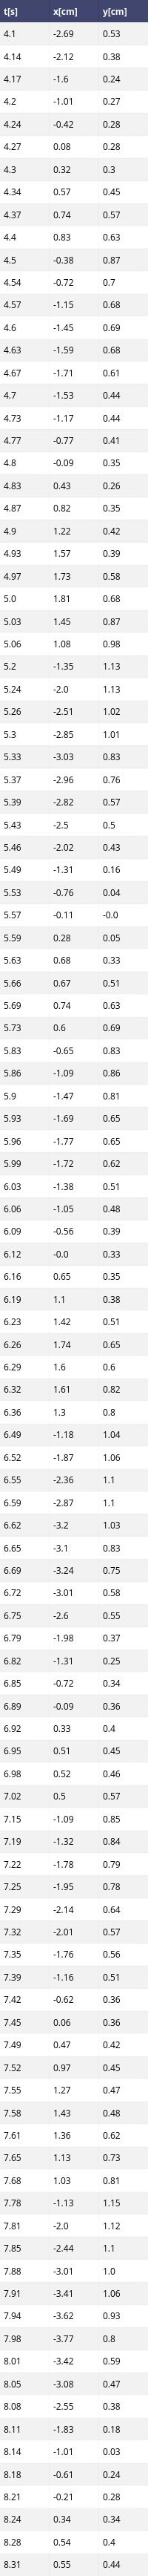
\includegraphics[scale=0.2,center]{t1_2}
	\caption{R(14.2cm) w(4.7098rad/s)}
\end{figure}
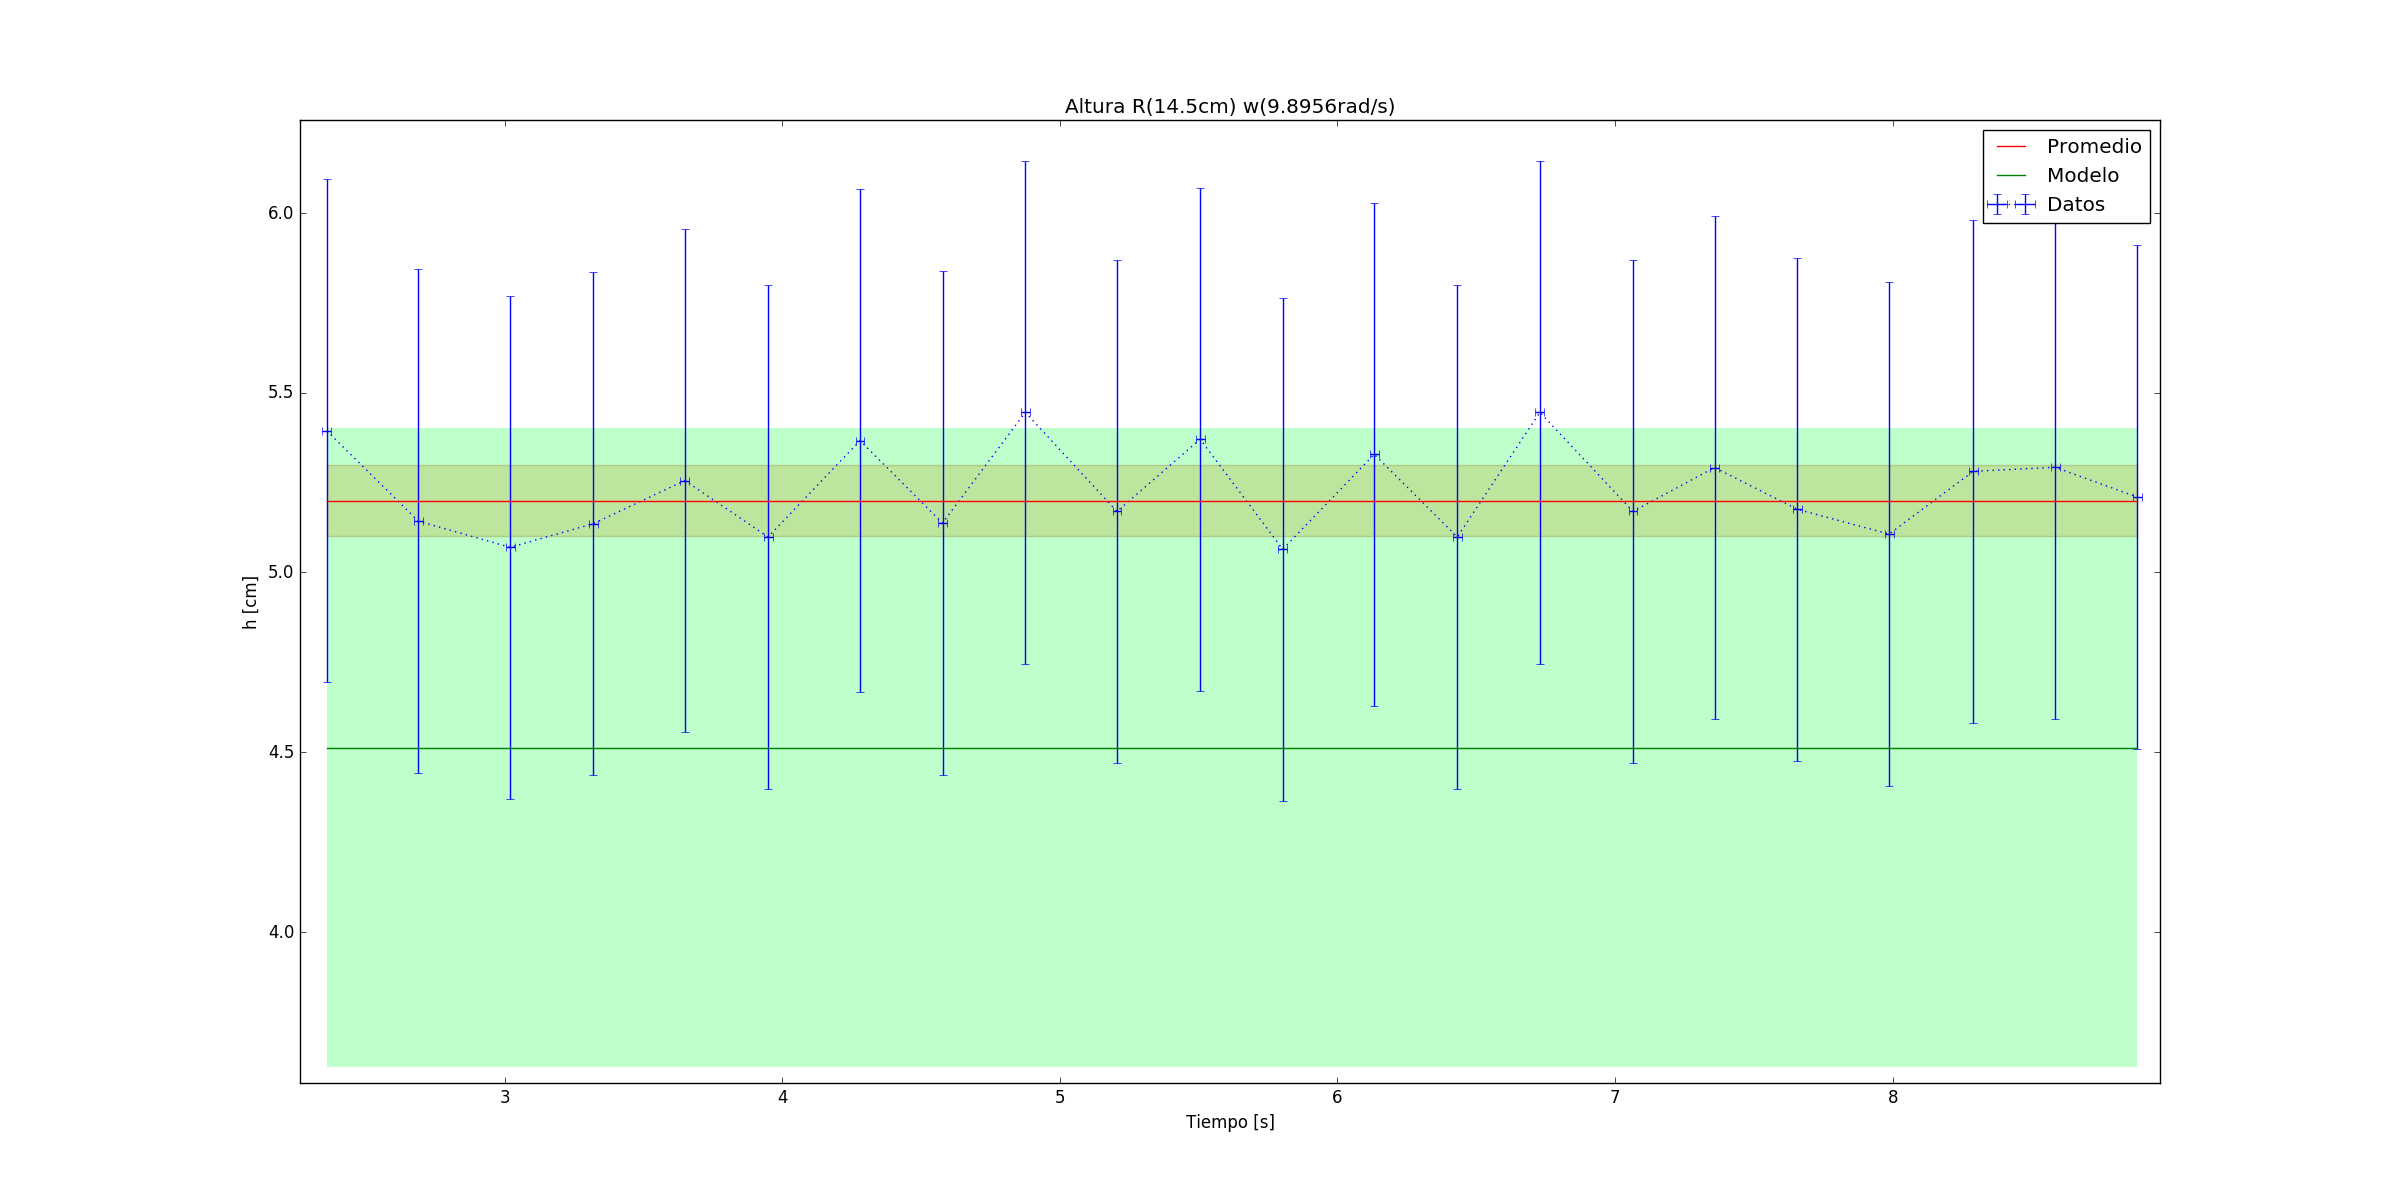
\includegraphics[scale=0.37,center]{1_3}
\begin{figure}
	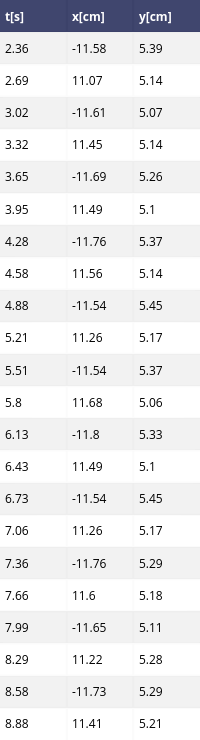
\includegraphics[scale=0.5,center]{t1_3}
	\caption{R(14.5cm) w(9.8956rad/s)}
\end{figure}
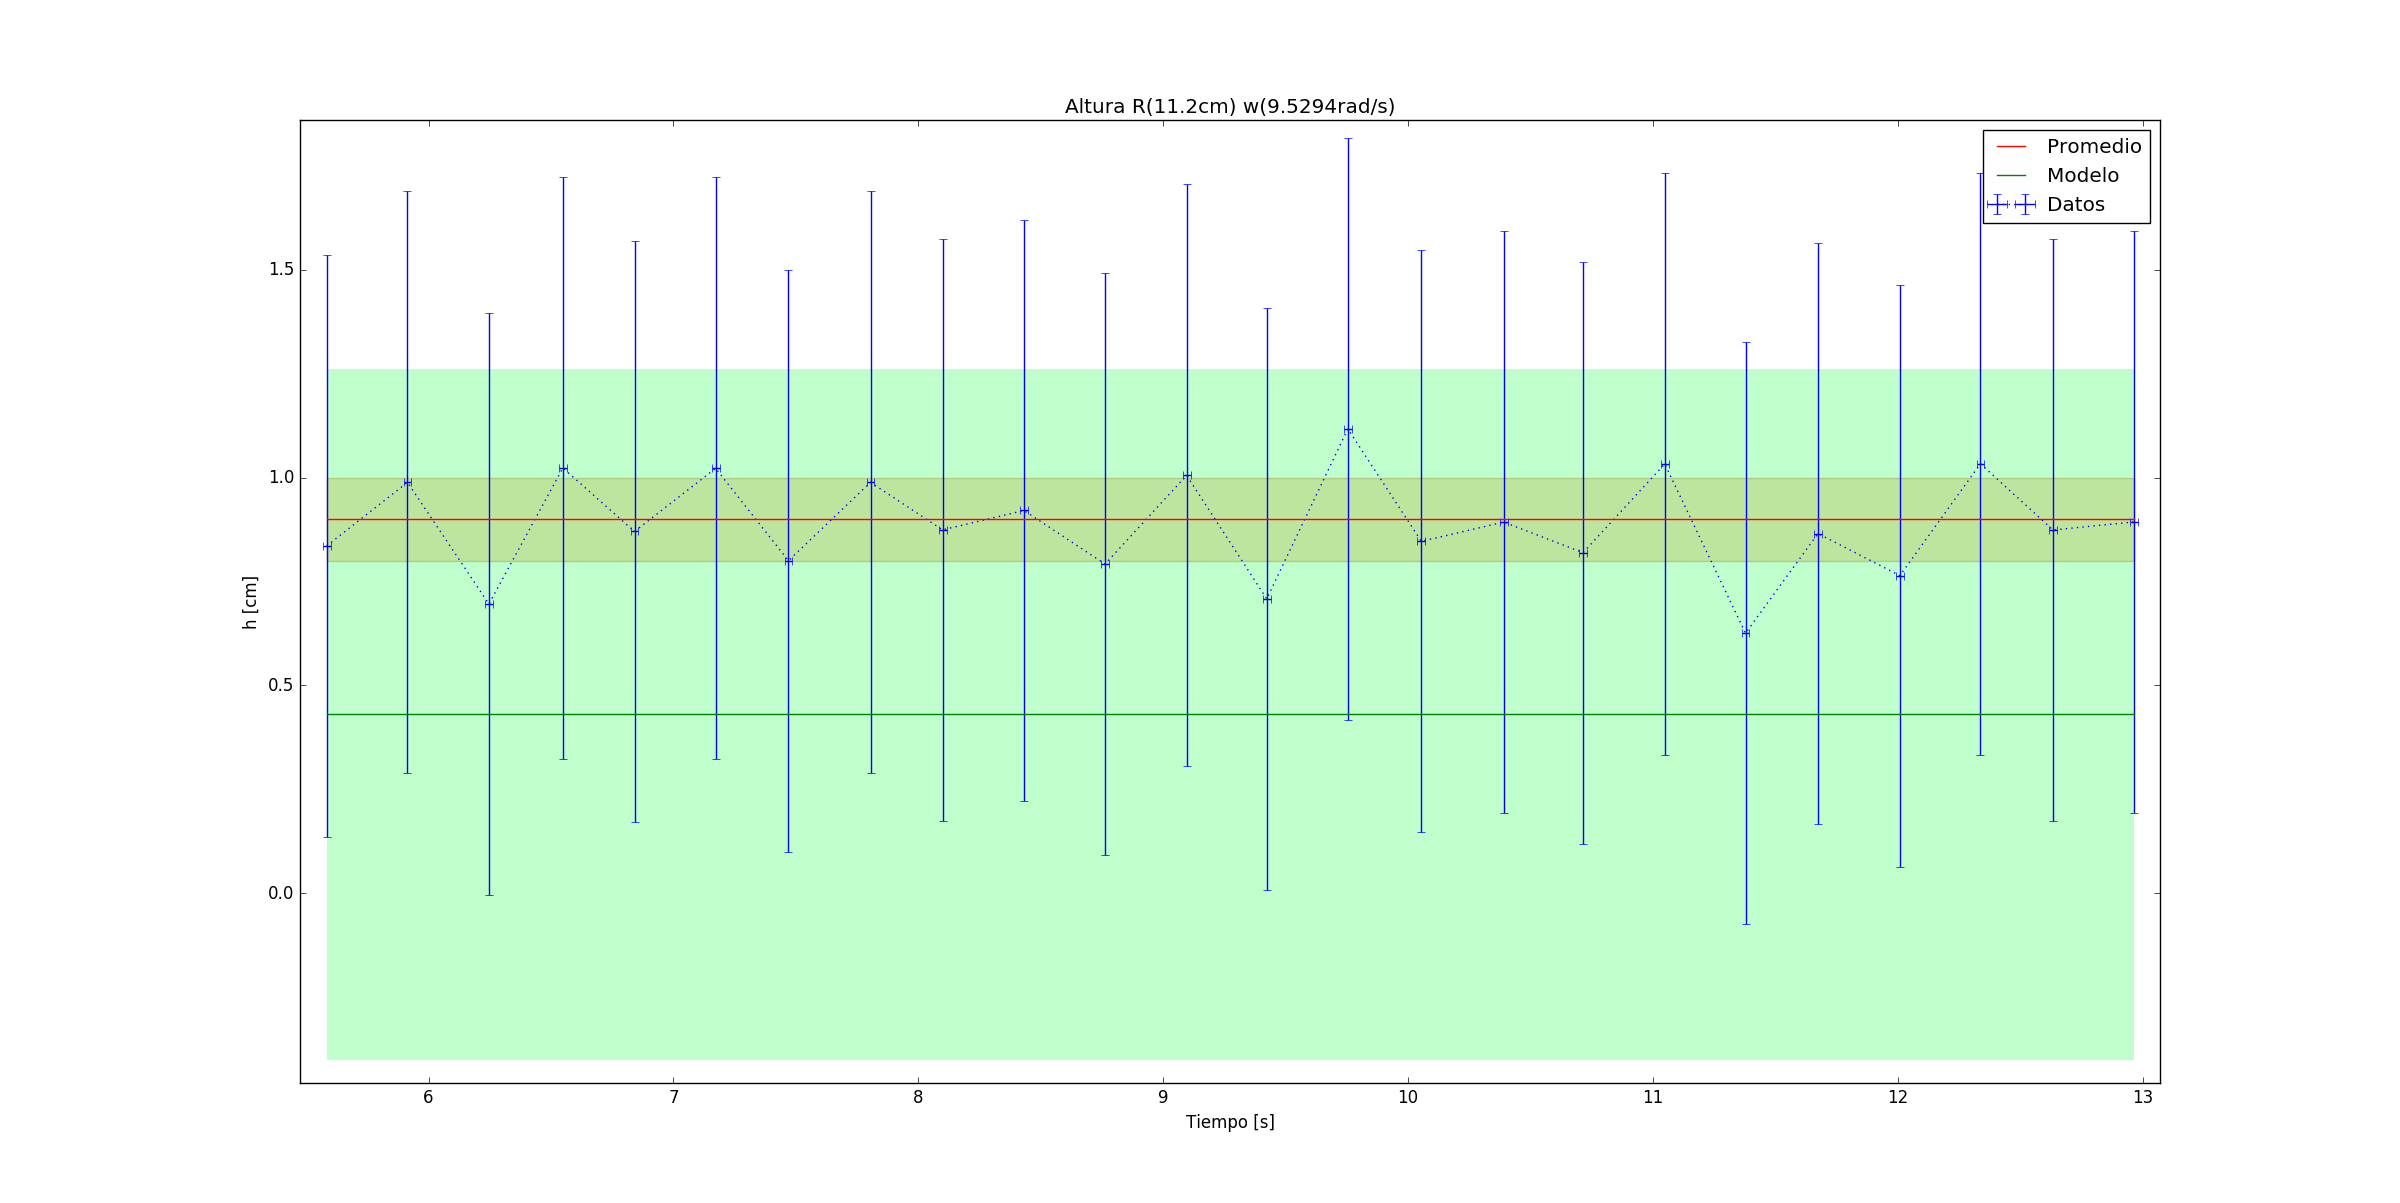
\includegraphics[scale=0.37,center]{2_1}
\begin{figure}
	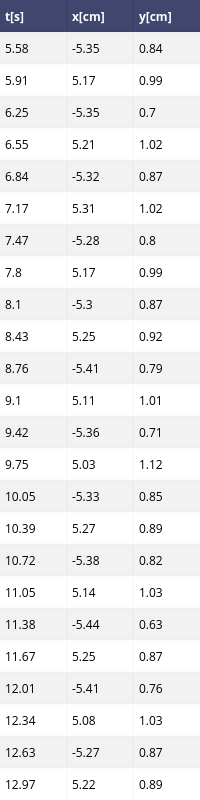
\includegraphics[scale=0.5,center]{t2_1}
	\caption{R(11.2cm) w(9.5294rad/s)}
\end{figure}
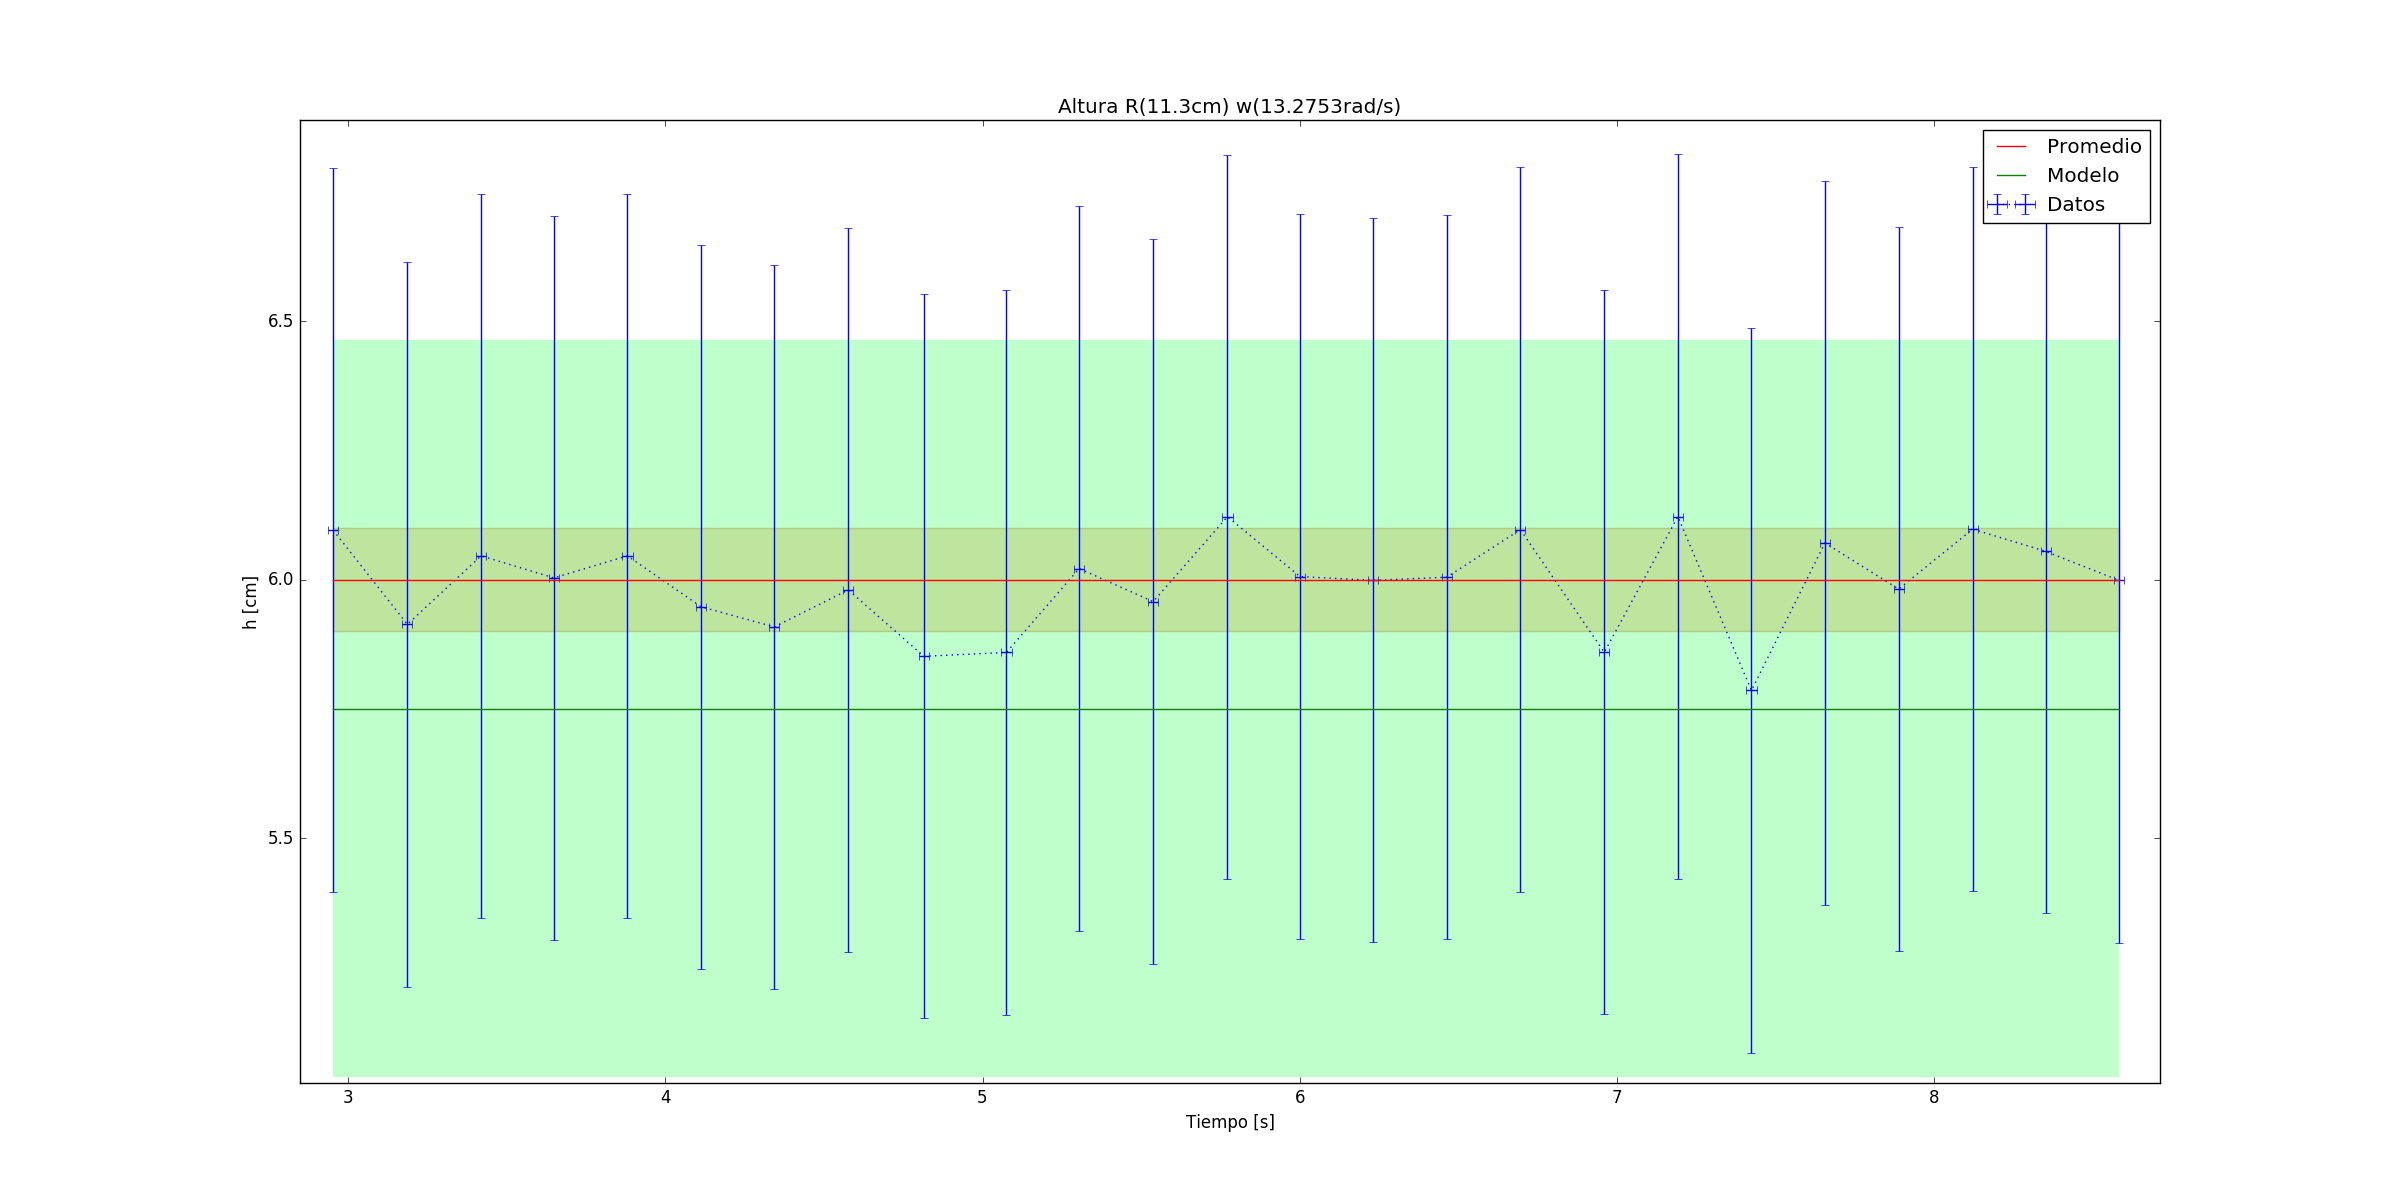
\includegraphics[scale=0.37,center]{2_2}
\begin{figure}
	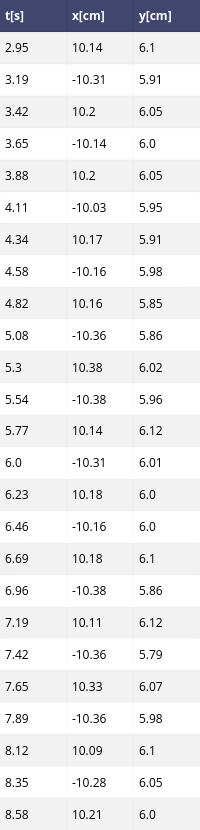
\includegraphics[scale=0.5,center]{t2_2}
	\caption{R(11.3cm) w(13.2753rad/s)}
\end{figure}
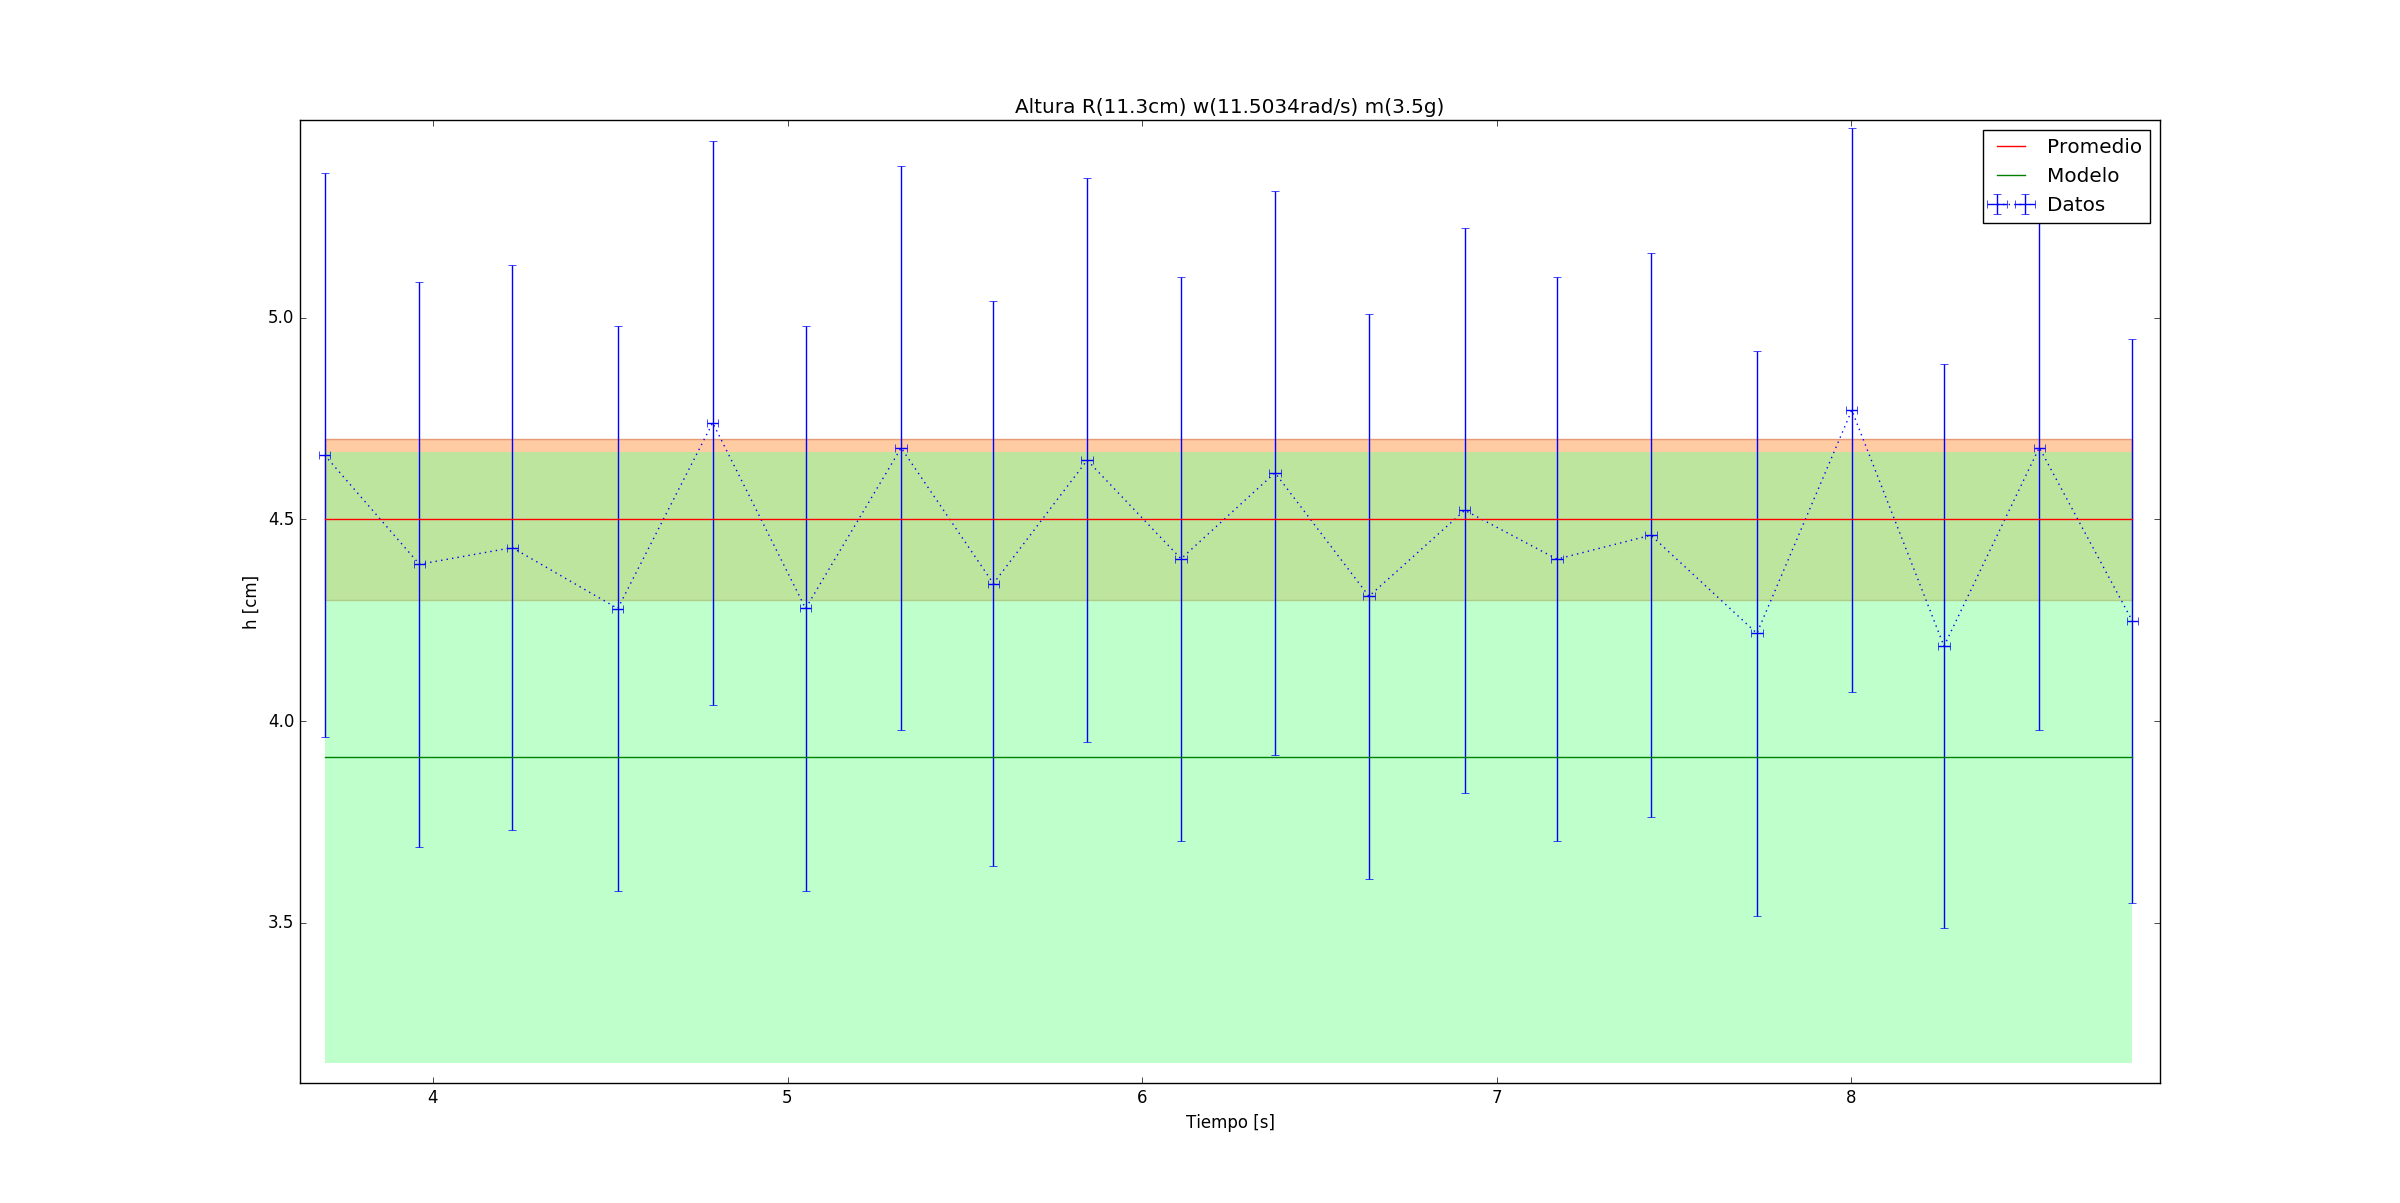
\includegraphics[scale=0.37,center]{2_3a}
\begin{figure}
	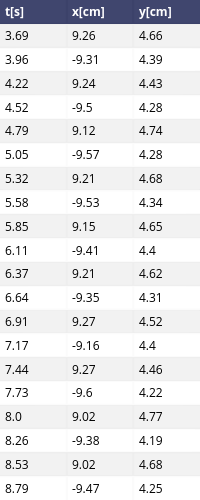
\includegraphics[scale=0.5,center]{t2_3a}
	\caption{R(11.3cm) w(11.5034rad/s) m(3.5g)}
\end{figure}
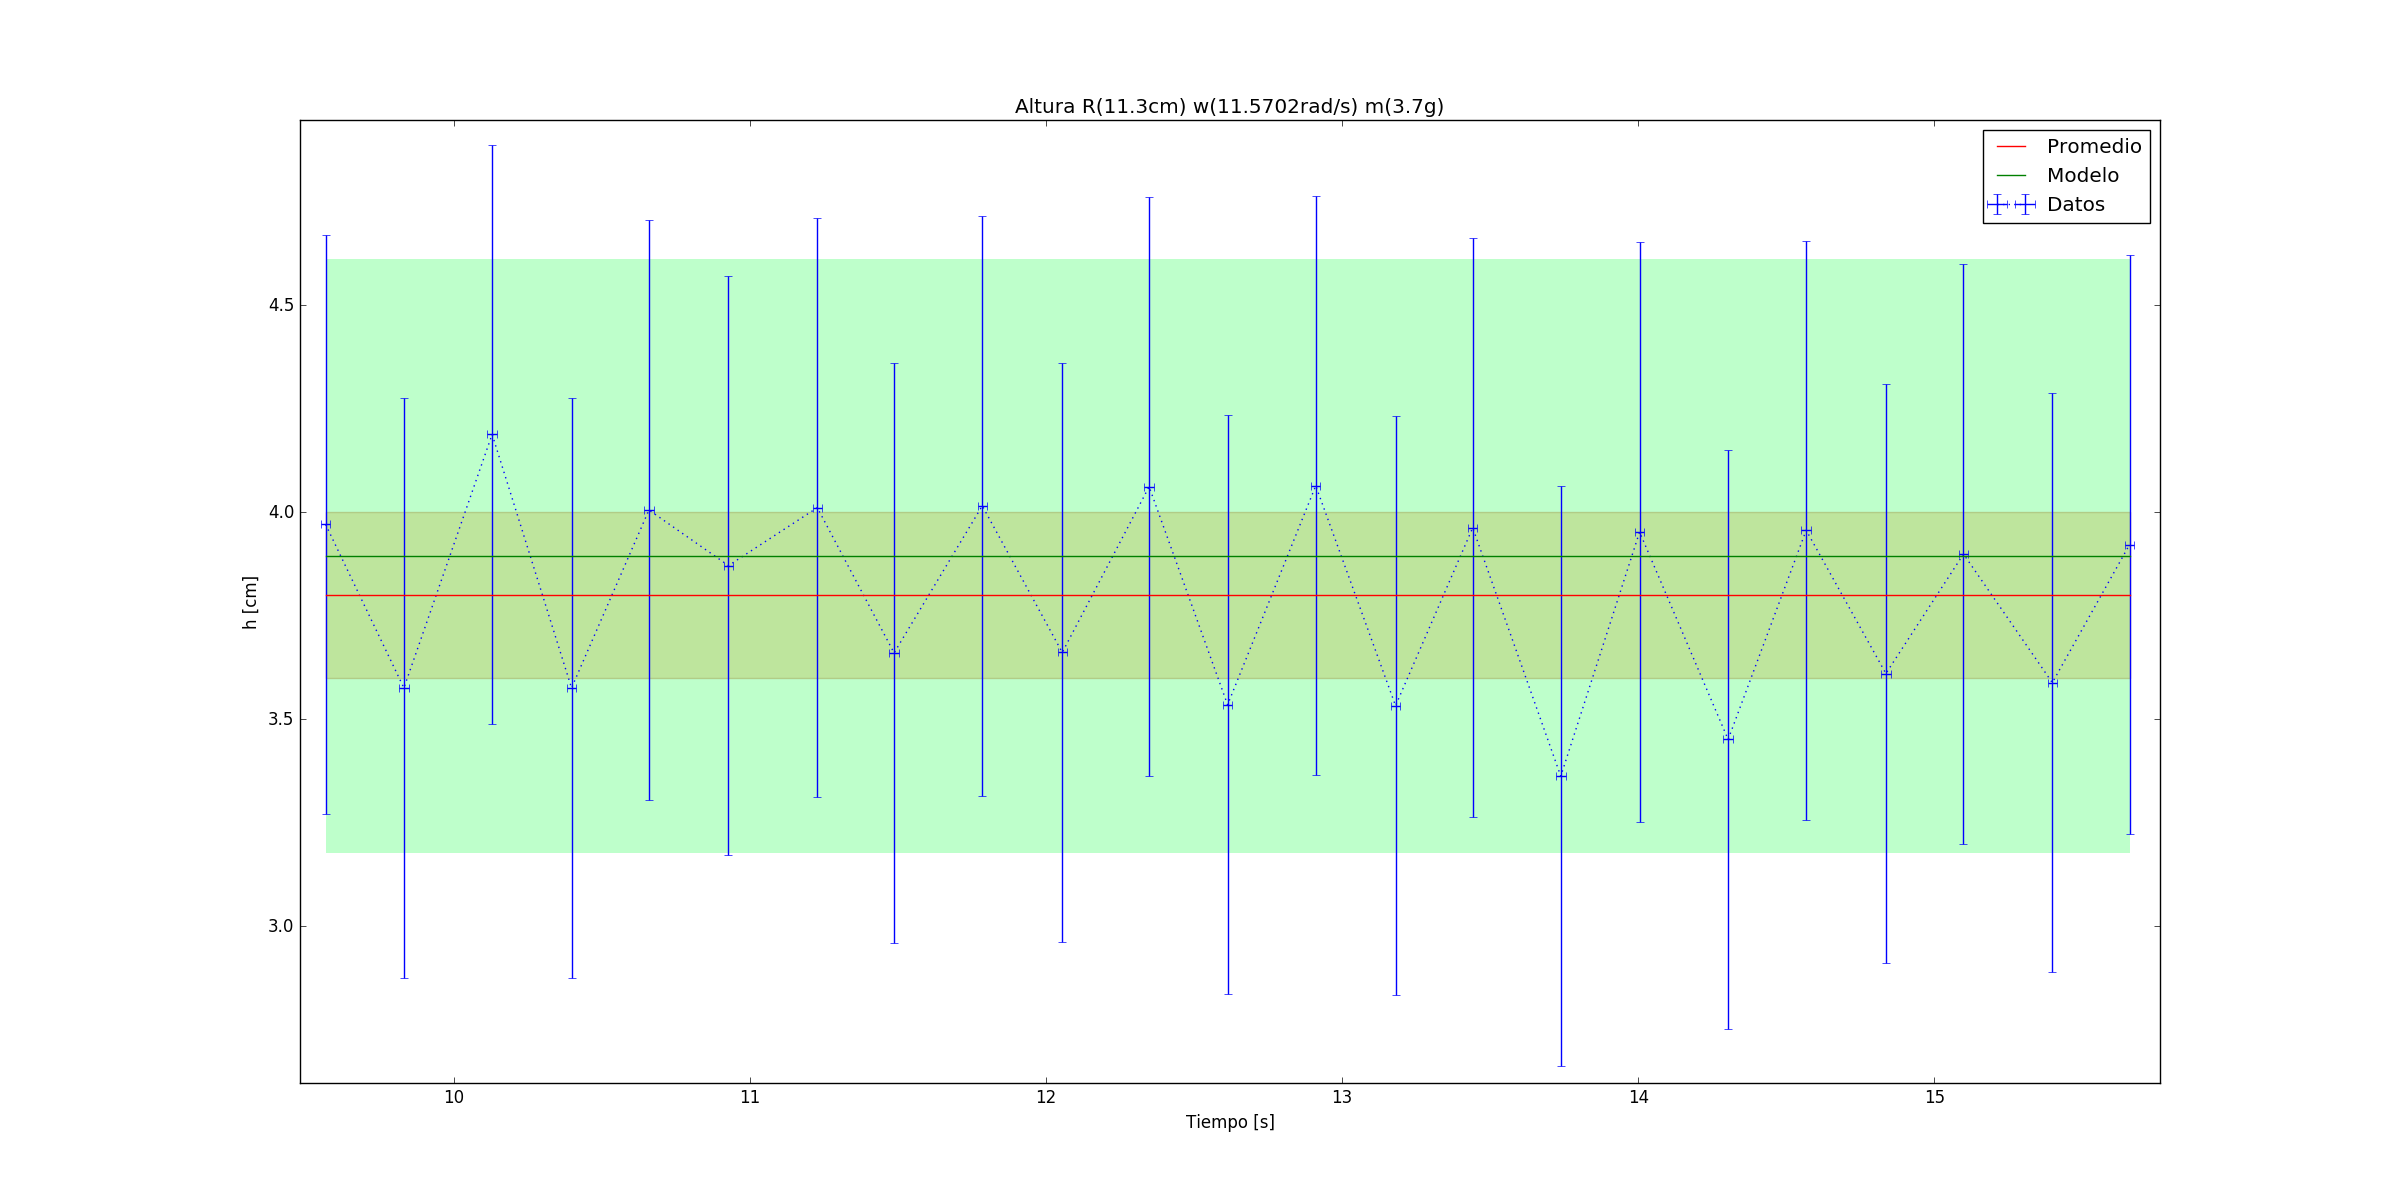
\includegraphics[scale=0.37,center]{2_3b}
\begin{figure}
	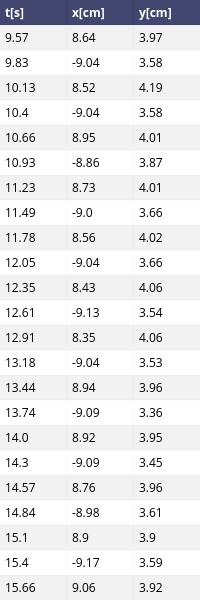
\includegraphics[scale=0.5,center]{t2_3b}
	\caption{R(11.2cm) w(11.5702rad/s) m(3.7g)}
\end{figure}
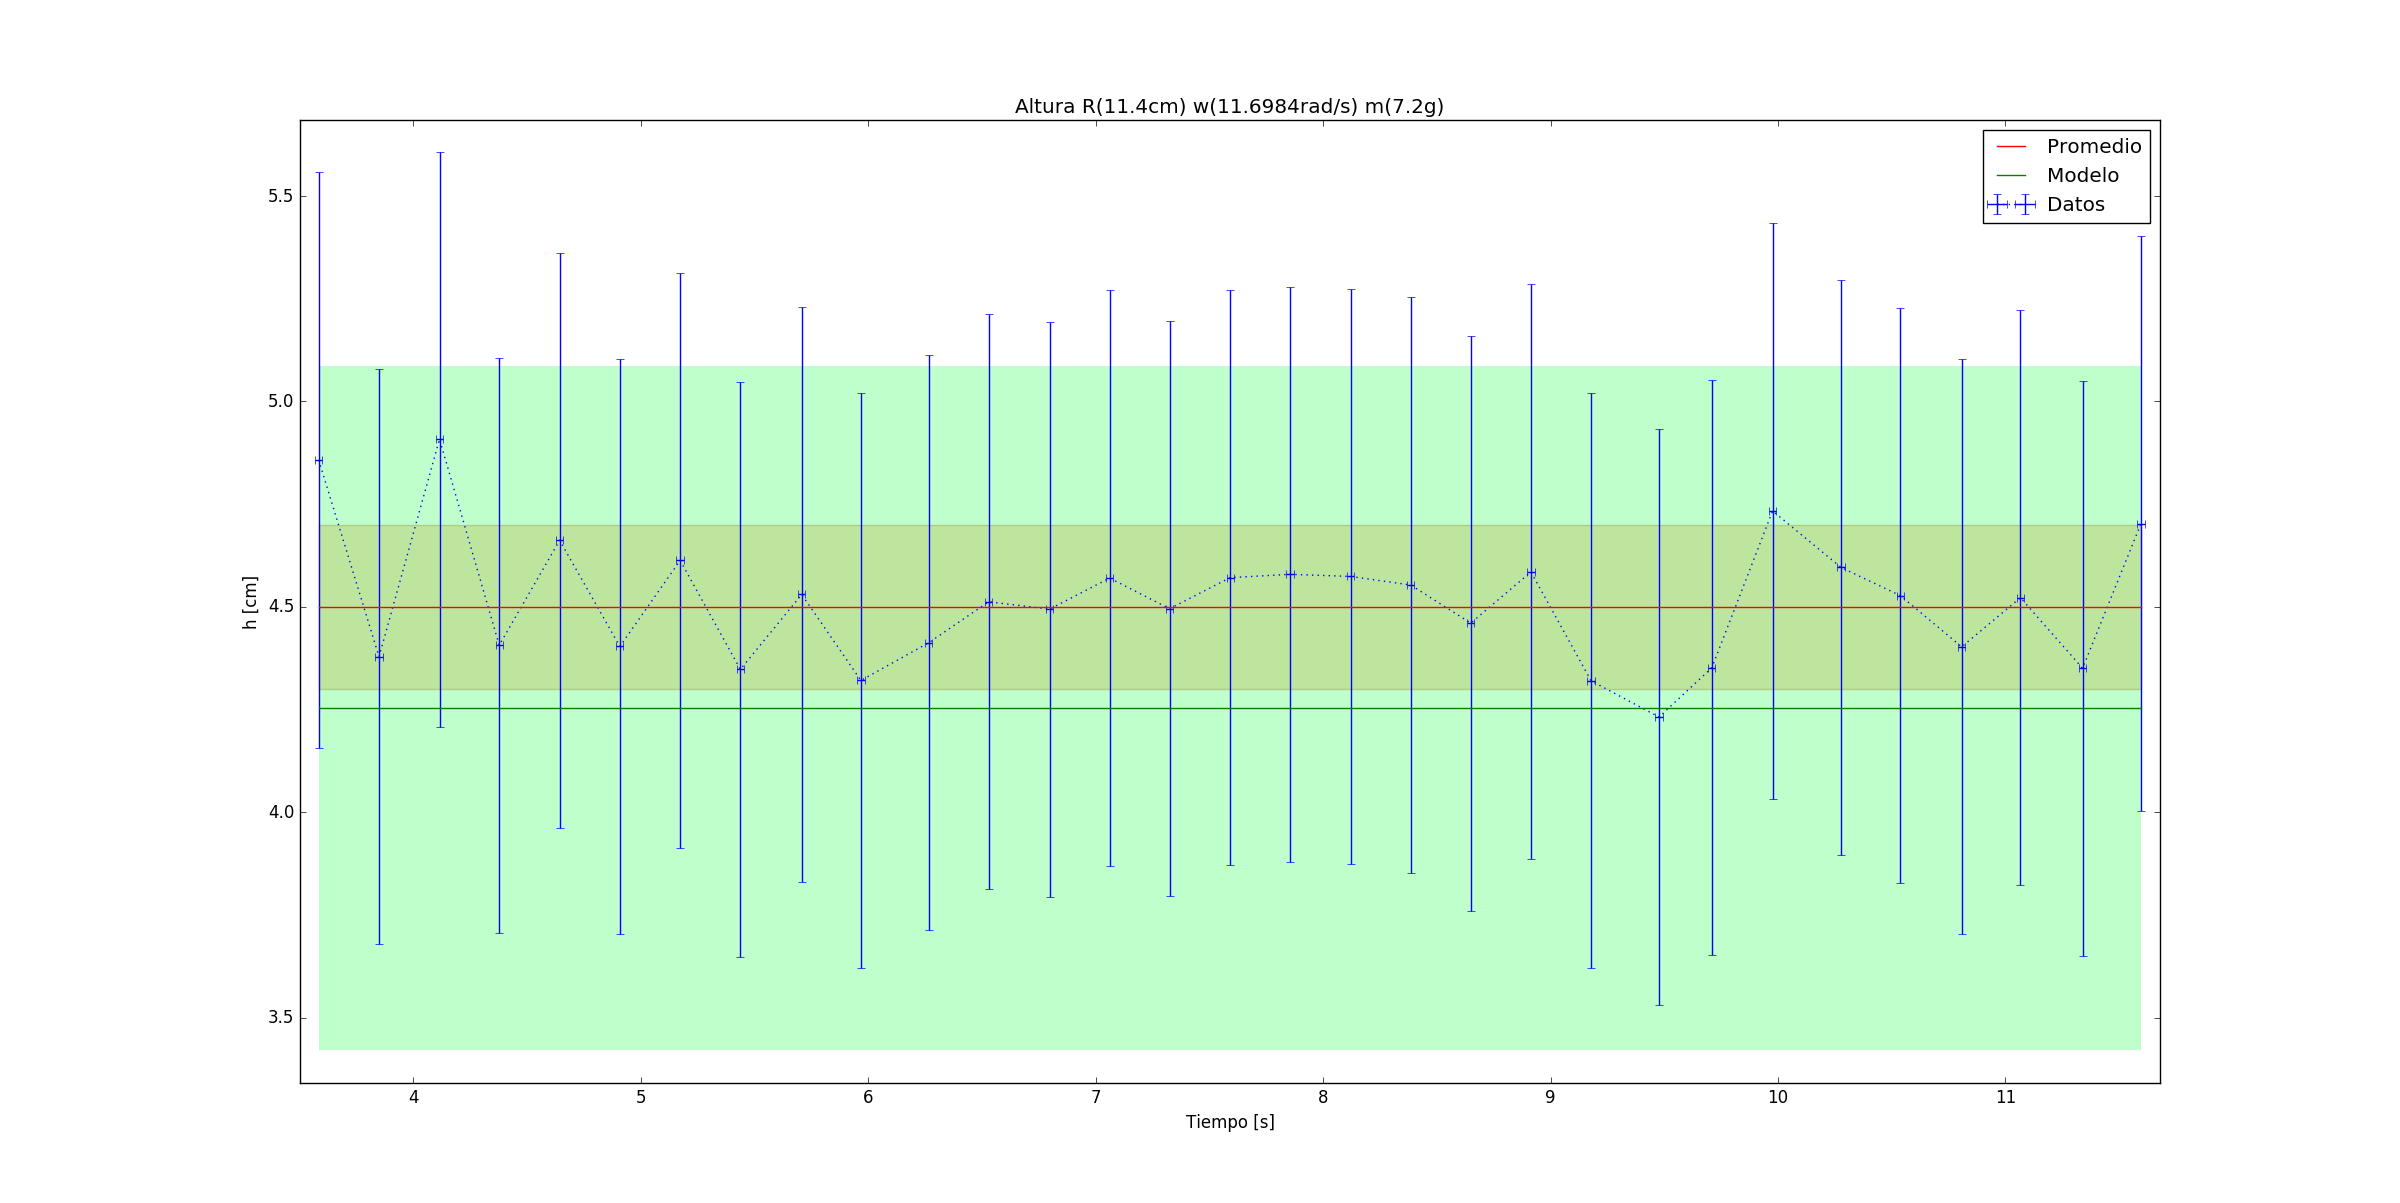
\includegraphics[scale=0.37,center]{2_3c}
\begin{figure}
	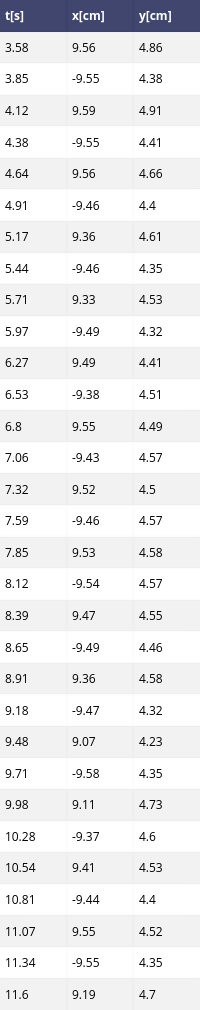
\includegraphics[scale=0.5,center]{t2_3c}
	\caption{R(11.4cm) w(11.6984rad/s) m(7.2g)}
\end{figure}
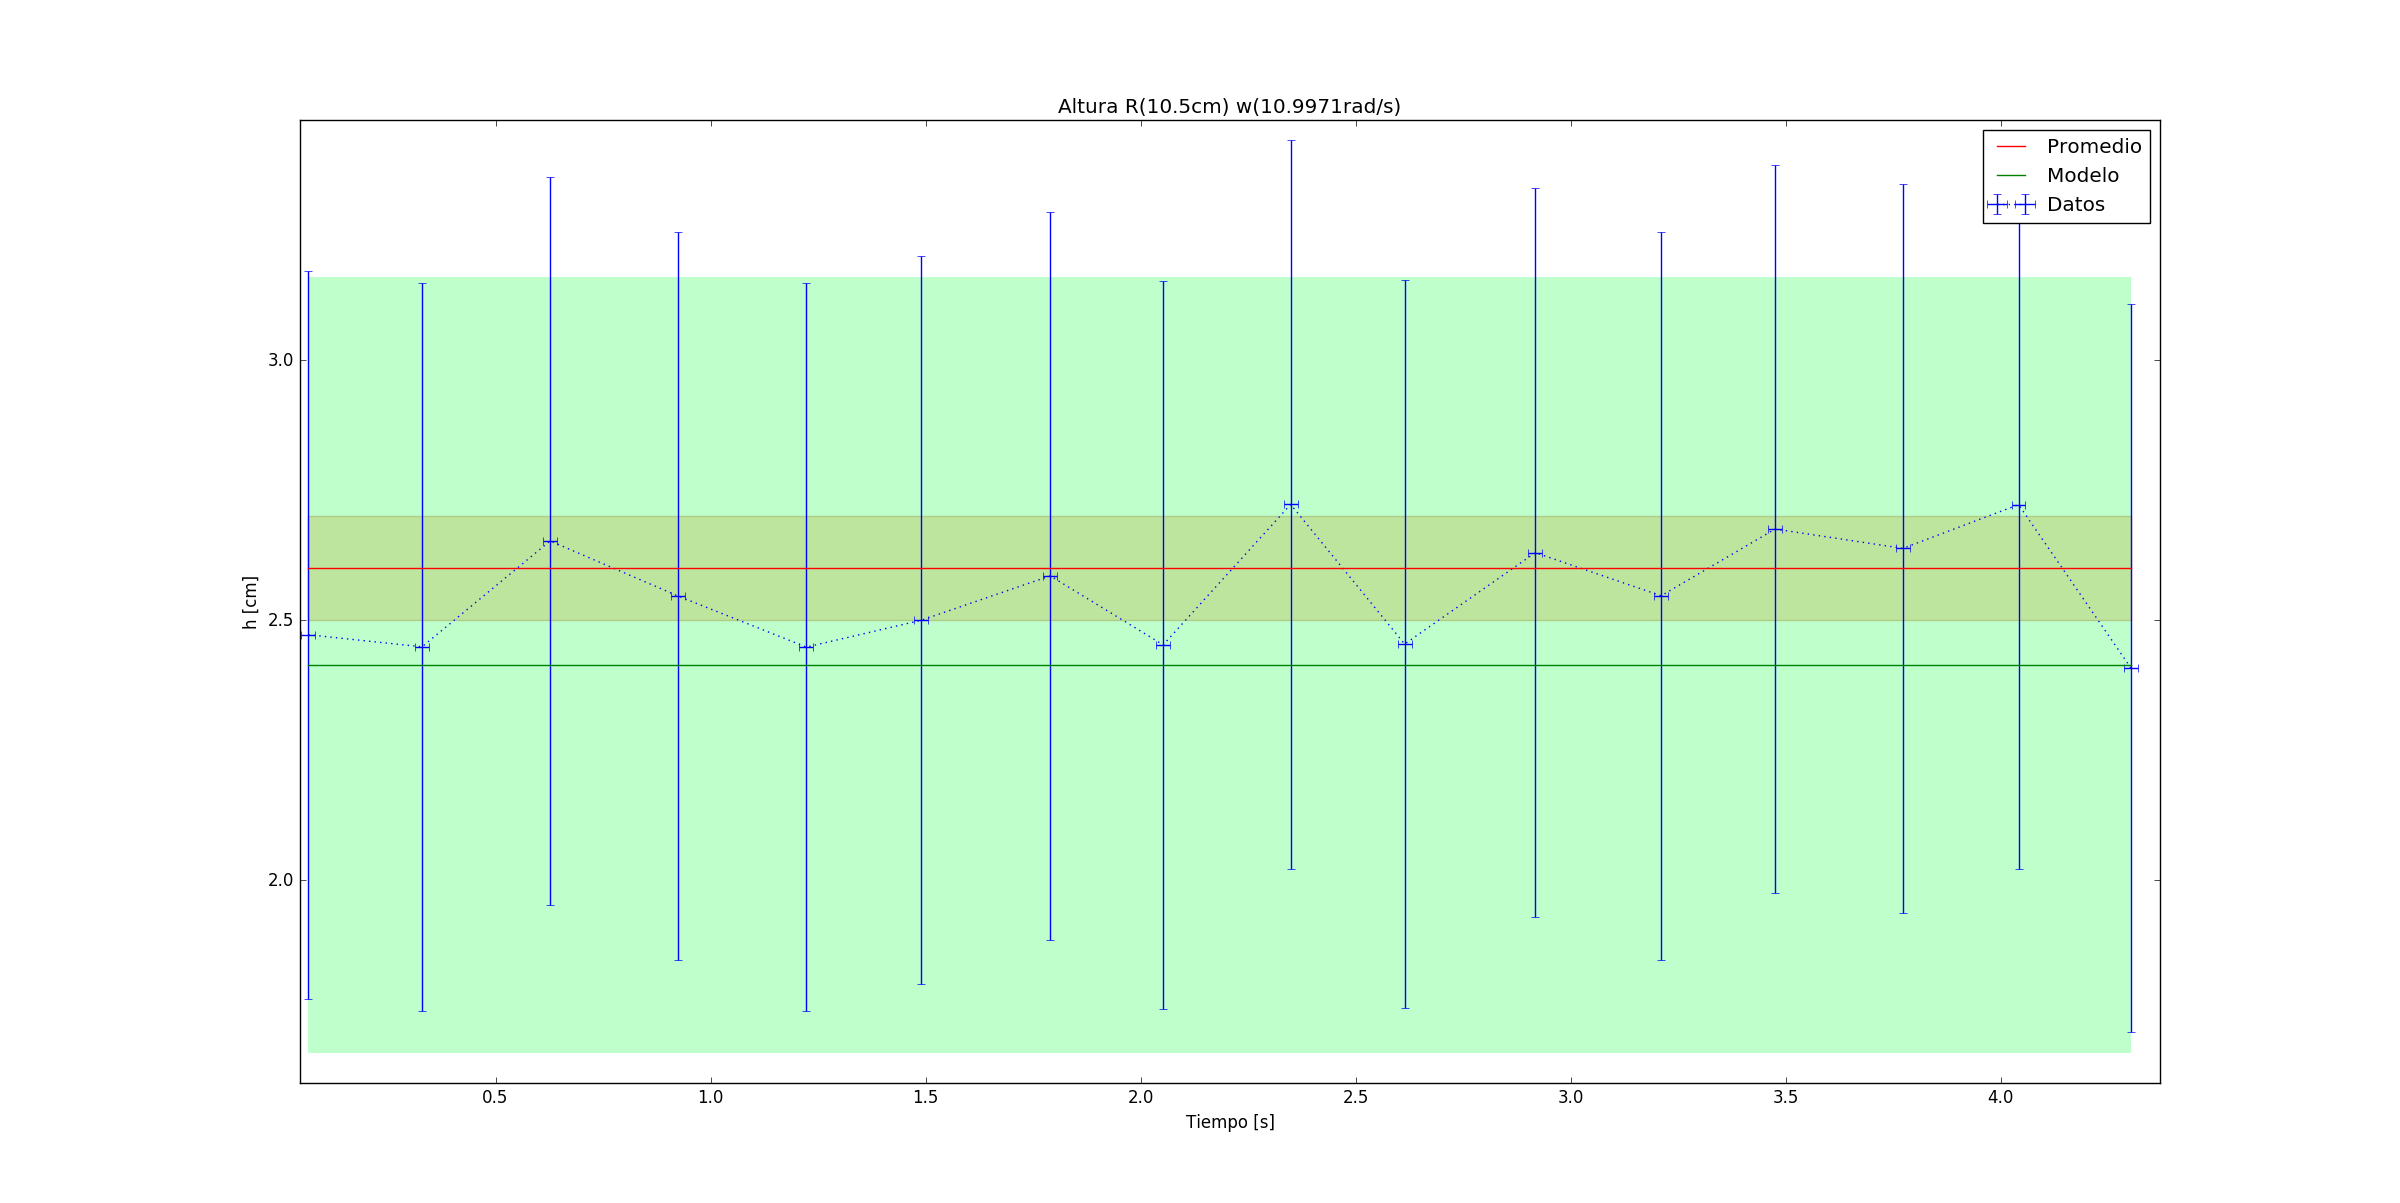
\includegraphics[scale=0.37,center]{3_1}
\begin{figure}
	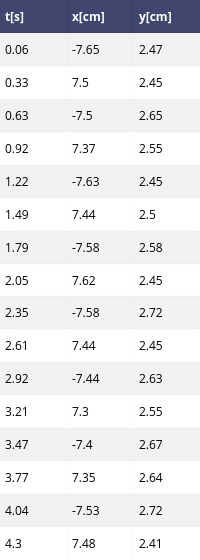
\includegraphics[scale=0.5,center]{t3_1}
	\caption{R(10.5cm) w(10.9971rad/s)}
\end{figure}
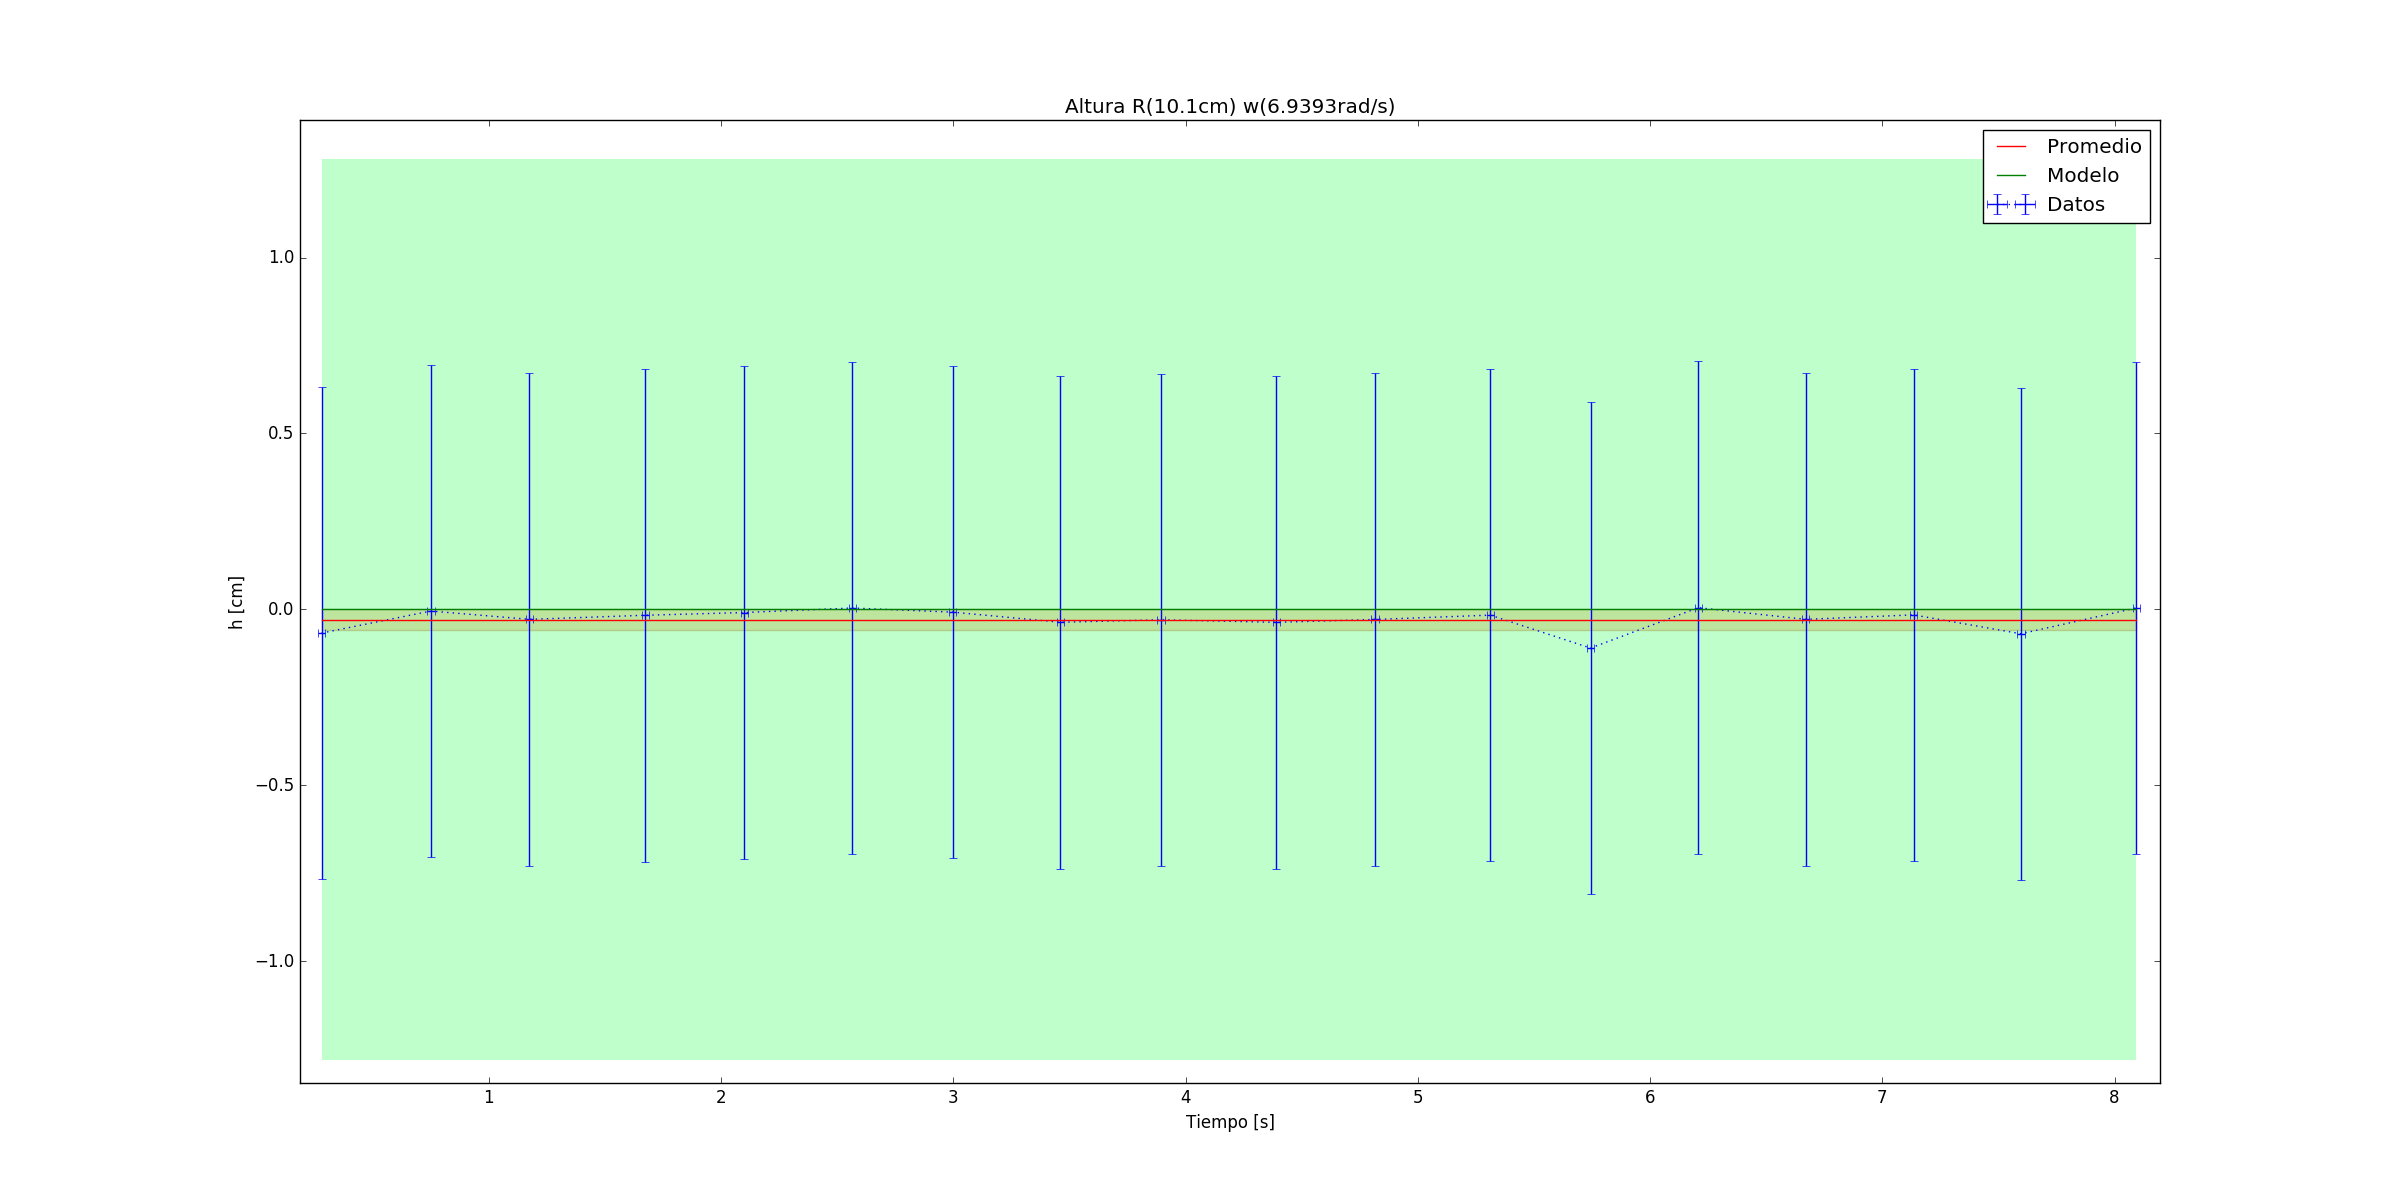
\includegraphics[scale=0.37,center]{3_2}
\begin{figure}
	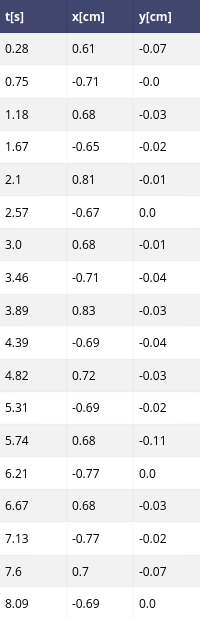
\includegraphics[scale=0.5,center]{t3_2}
	\caption{R(10.1cm) w(6.9393rad/s)}
\end{figure}
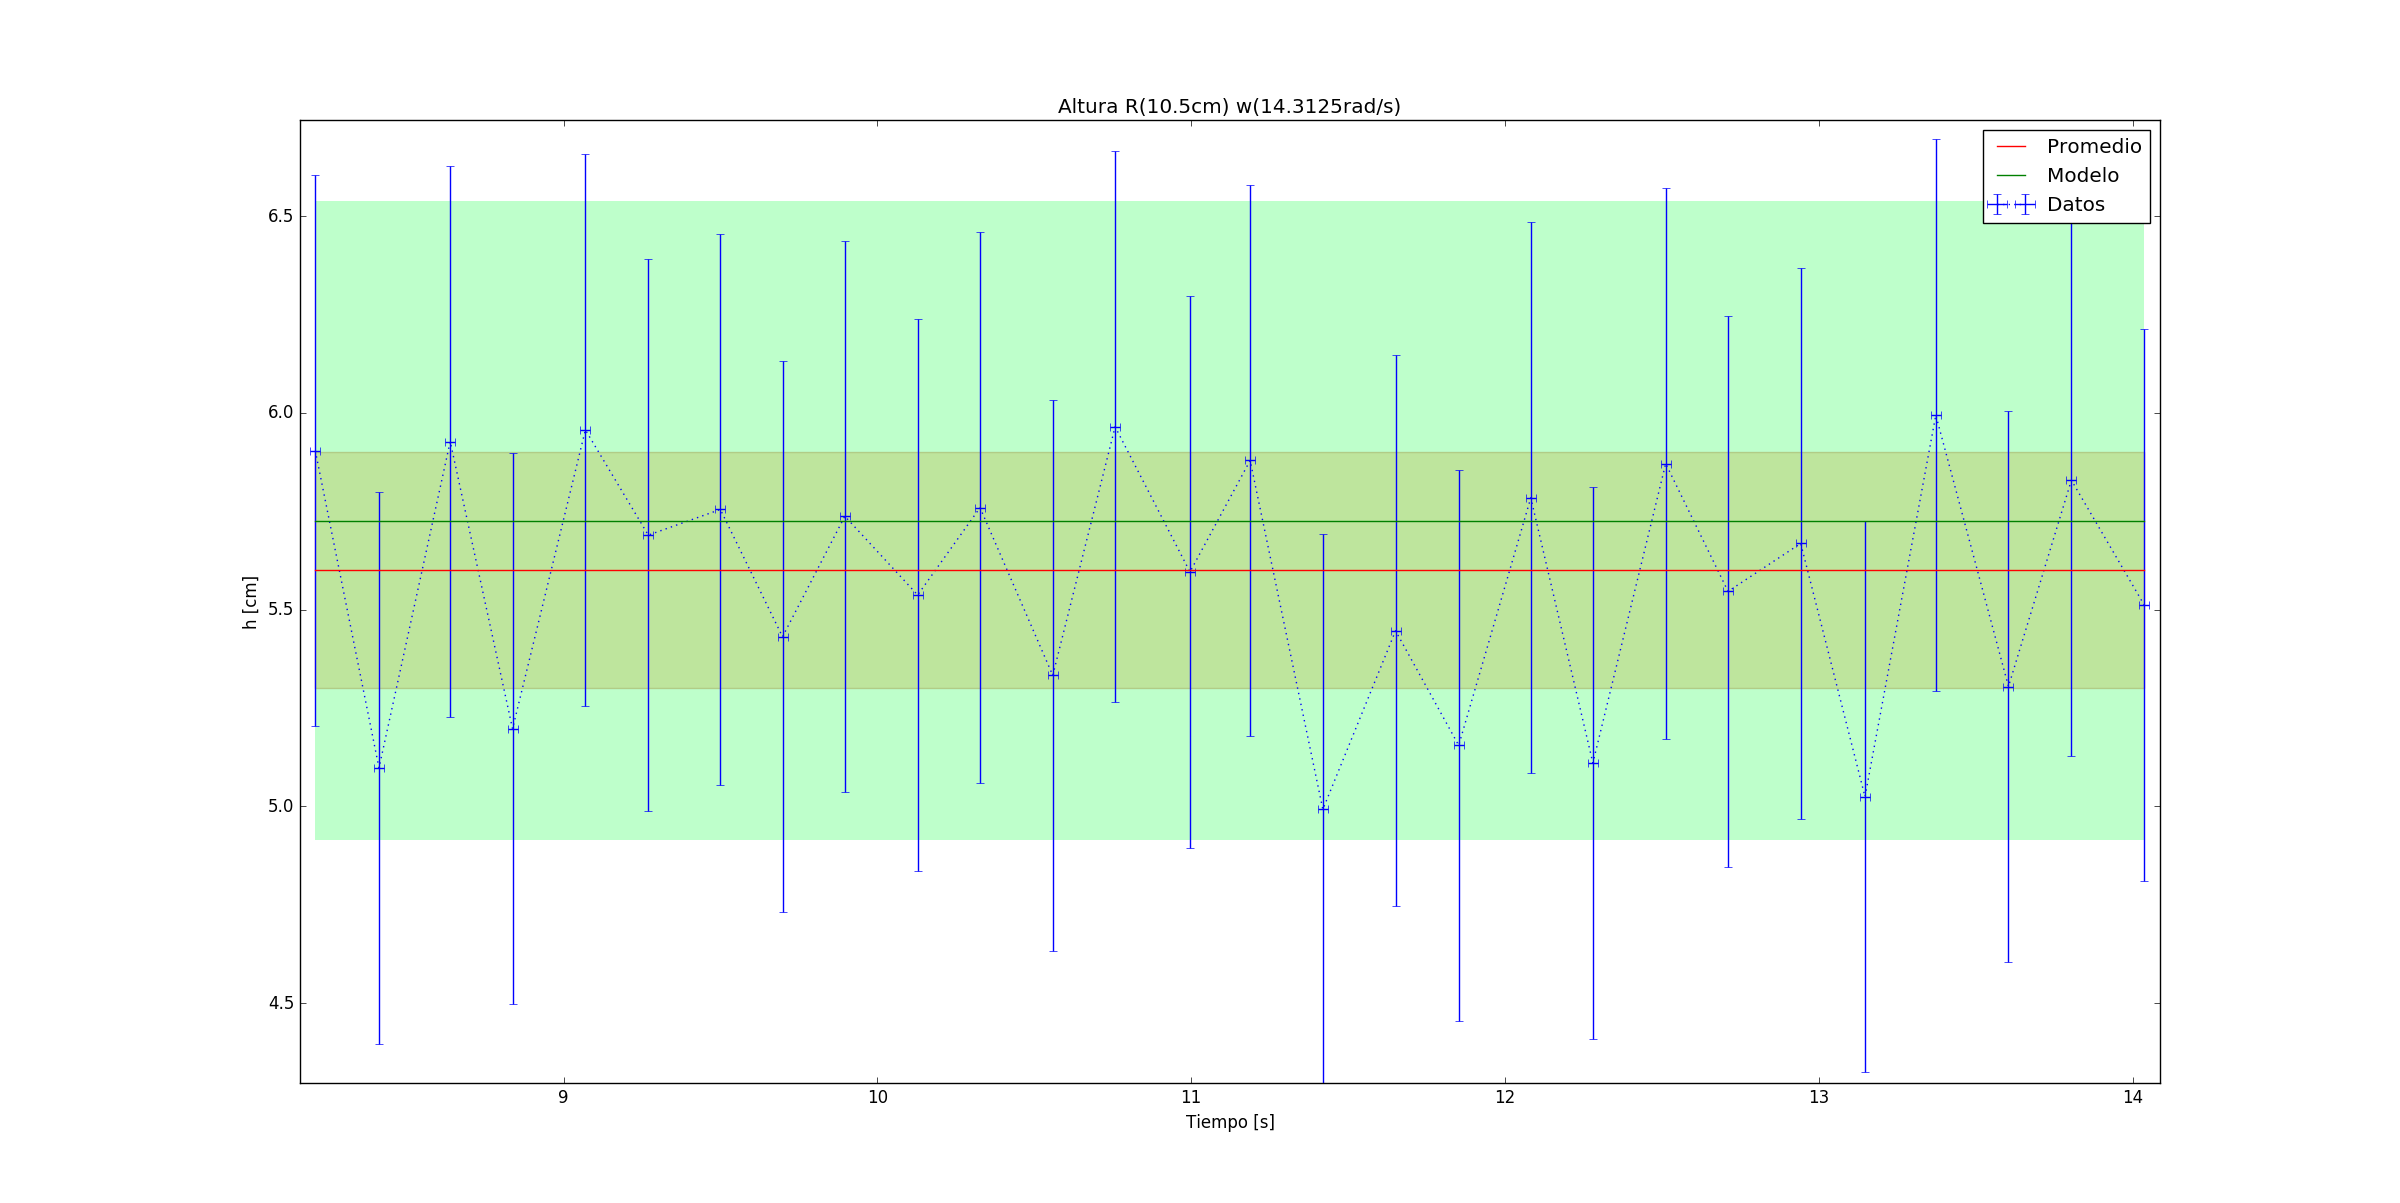
\includegraphics[scale=0.37,center]{3_3}
\begin{figure}
	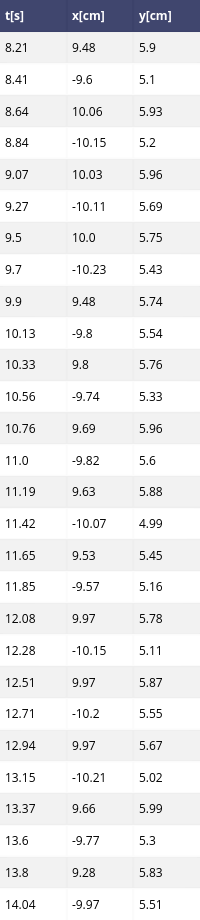
\includegraphics[scale=0.5,center]{t3_3}
	\caption{R(10.1cm) w(14.3125rad/s)}
\end{figure}

A continuación la tabla con las respectivas velocidades angulares críticas que caracterizan a los puntos de equilibro, obtenidas mediante la fórmula $\sqrt{\frac{g}{R}}$ para cada radio obtenido.

\begin{figure}
	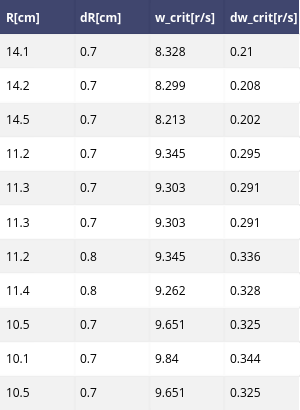
\includegraphics[scale=0.5,center]{w_crit}
	\caption{Velocidades angulares críticas}
\end{figure}

Por último una tabla que resume todas las mediciones. Tomando en cuenta el radio de la cricunferencia, la masa de la canica, el promedio del periodo obtenido, la velocidad angular obtenida, el promedio de la altura máxima medida, junto con su desviación estándar y la altura esperada por el modelo, junto con el error asociado al error de los parámetros que lo definen.

\begin{figure}
	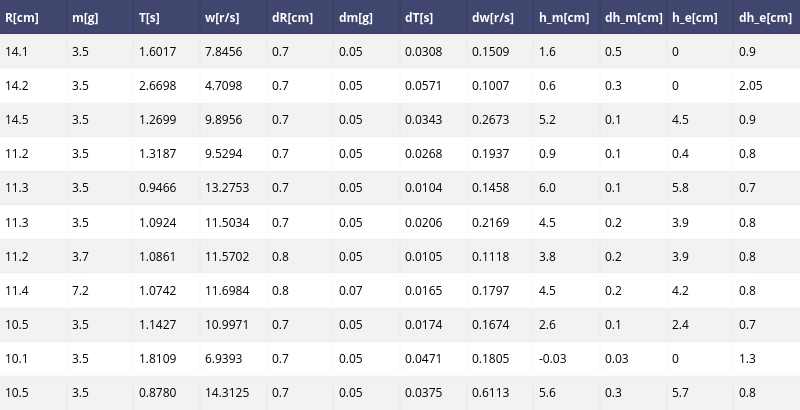
\includegraphics[scale=0.5,center]{all}
	\caption{Tabla de resultados generales}
\end{figure}

\section{Discusión}

A simple vista los resultados parecen ser positivos. En 10 de 11 experimentos, el promedio de la altura medida entra dentro del margen de error de la altura esperada por el modelo obtenido, aunque sólo en 3 de ellos el valor de la altura esperada entra dentro del margen dado por la desviación estándar de la muestra de datos. En 8 de los 11 experimentos, el valor promedio obtenido queda por arriba del esperado. Ésto nos dice que, aunque los resultados validan el modelo, probablemente hubo un error sistemático que no fue tomado en cuenta que hizo que la muestra de datos tuviera un valor mayor al esperado, o bien, puede que las fotocompuertas hubieran estado descalibradas de alguna forma, provocando que las mediciones de las velocidades angulares sean menor a las reales, lo que se ve traducido en una altura esperada menor a la que fue medida.

El único experimento que arrojó un resultado negativo fue el de la primera gráfica (R(14.1cm) w(7.8456rad/s)), que tenía una velocidad angular medida menor a la velocidad angular crítica (8.328rad/s), por lo que se esperaría que el punto de equilibrio fuera en la base, en h=0. En cambio, si observamos la gráfica, podemos ver que, incluzo con intervalos de tiempo de medición de medio periodo, la altura de la canica realiza oscilaciones alrededor de su promedio (1.6cm). A éste comportamiento se le podría ajustar una función senoidal, que describe el movimiento de un oscilador armónico con periodos bastante grandes (entre 8 y 13 segundos) , que era exactamente lo que se esperaba para velocidades angulares más grandes que la velocidad angular crítica, con una pequeña perturbación inicial, para variaciones de alturas pequeños. Por el contrario, la velocidad angular medida fue menor a la crítica, por lo que ese comportamiento se esperaba alrededor de la base del aro. Así, aunque no podemos concluir nada satisfactorio con éste experimento, la validez del modelo que nos proporcionan los demás experimentos nos da razones para creer que simplemente hubo un error de medición de la velocidad angular de al menos 0.5 rad/s, pues sería la diferencia mínima necesaria para que la velocidad angular sea mayor a la crítica.

El segundo experimento, el de la gráfica R(14.2cm) w(4.7098rad/s), tuvo el comportamiento de oscilador armónico mencionado en el párrafo anterior, pero ahora sobre la base del aro. La gráfica puede mostrar que el movimiento fue alrededor de un punto más alto, pero un vistazo al video "v2arogrande", muestra que la canica claramente oscila alrededor de la base. Éste se debe a la dificultad en el posicionamiento del origen. Pero principalmente a la forma en la que se hicieron las mediciones, ya que el origen se puso a una altura dada por el radio de la canica, por lo que ninguna medición podía tener alturas negativas. Así, aunque la oscilación sea con respecto al origen, la altura alrededor de la cual oscila siempre será mayor que cero. No hay un error sistemático provocado por la colocación del origen debajo por donde debía estar, pues se puede observar que hay un par de mediciones que si llegan a ser exactamente cero. Por otra parte, el comportamiento mismo de la oscilación es muy interesante. Ya se mencionó anteriormente que habría un error de perspectiva devido a que las mediciones se tomaron en intervalos "continuos" (más bien discretos, dados por la cámara). Los huecos del conjunto de datos resultan ser bastante útiles, pues a partir de ellos podemos conocer el punto en el cual no hay error de perspectiva, el punto medio entre dichos huecos. Éste punto, a exepción de un muy pequeño error, coincide con el promedio de los datos, lo que nos dice que cada que el aro se alineaba con la cámara, la canica estaba a la misma altura. Lo mejor de todo es el patrón característico de la ubicación de dichos huecos con respecto a la evolución del movimiento de la canica: los huecos siempre se ubican en la misma posición de la forma senoidal del movimiento, siempre justo antes de llegar a la altura máxima. Ésto nos dice claramente que se pudo replicar un movimiento oscilatorio de la canica con un periodo de oscialción igual al del giro del aro. Uno podría decir que éste movimiento no corresponde al de un oscilador armónico, debido a que las alturas máximas se intercalan (primero hay una cresta grande, luego una pequeña, etc), pero debemos recordar que éste conjunto de datos en específico no puede ser interpretado de ésa forma, pues existe un error de perspectiva, donde de hecho, por la ubicación de los huecos del conjunto de datos, el error de perspectiva es mayor en las crestas.

De los demás conjuntos de datos sólo se puede decir que la altura esperada y la altura medida fue satisfactoria con respecto al margen de error obtenido. Puede que haya habido pequeñas oscilaciones armónicas en éstos, pero no fueron aparentes ni en el video ni en las gráficas. Puede que el periodo de oscilación no coincidiera con el de la rotación del aro, por lo que al haber tomado datos cada media vuelta, los datos obtenidos no formarían un patrón de oscilador armónico, como así se observa. Por otro lado, las gráficas 3,4,6,7 y11 sí muestran patrones de alturas alternantes entre cada medición, pero esto se debe a algún error en la inclinación de los ejes (fenómeno mencionado anteriormente en la metodología). Puede que un movimiento oscilatorio con un mismo periodo haya tenido efecto en algunos, pero es más probable que el error de los ejes haya producido un efecto mayor, por lo que no se puede conlcuir nada satisfactoriamente de ésos experimentos en cuanto a que si los puntos esperados son puntos de equilibrio que a pequeñas variaciones forman osciladores armónicos.

Se tiene que hacer una mención especial al análisis cuidadoso realizado en tracker, ya que una recopilación de datos preeliminar y a ciegas mostraba errores sistemáticos de hasta 3 o 4 centímetros entre el modelo y los datos, arrojando conclusiones insatisfactorias con un error sistemático. Afortunadamente ése no fue el caso.

\begin{thebibliography}{9}
\bibitem{Gravedad en la ciudad de méxico} %Para páginas de internet 
Cálculo de la aceleración de la gravedad,
\\\texttt{http://www.metas.com.mx/utilerias/calculoacelgravedad.php}
\end{thebibliography}

\end{document}